% Memoria del proyecto: Optimización multiobjetivo de rutas turísticas en Gran Canaria
% Compilar desde esta carpeta:  pdflatex main.tex  (dos veces, para referencias cruzadas)
% Las figuras se leen de ../output/ (generadas por el código del repositorio).
\documentclass[11pt,a4paper]{article}

\usepackage[spanish,es-tabla,es-noshorthands]{babel}
\usepackage[utf8]{inputenc}
\usepackage[T1]{fontenc}
\usepackage{lmodern}
\usepackage{microtype}
\usepackage[a4paper,margin=2.5cm]{geometry}
\usepackage{amsmath,amssymb}
\usepackage{graphicx}
\usepackage{booktabs}
\usepackage{tabularx}
\usepackage{array}
\usepackage{multirow}
\usepackage{caption}
\usepackage{subcaption}
\usepackage{float}
\usepackage{enumitem}
\usepackage{xcolor}
\usepackage{algorithm}
\usepackage{algpseudocode}
\usepackage[round,authoryear]{natbib}
\usepackage[hidelinks]{hyperref}

\graphicspath{{../output/}{../output/figuras/}}
\setlist{itemsep=2pt,topsep=4pt}
\setlength{\emergencystretch}{2.5em}
\captionsetup{font=small,labelfont=bf}
\renewcommand{\algorithmicrequire}{\textbf{Entrada:}}
\renewcommand{\algorithmicensure}{\textbf{Salida:}}
\floatname{algorithm}{Algoritmo}
\renewcommand{\listalgorithmname}{Lista de algoritmos}

% Notación
\newcommand{\Tmax}{T_{\max}}
\newcommand{\code}[1]{\texttt{#1}}

\title{\textbf{Optimización multiobjetivo de rutas turísticas en Gran Canaria}\\[4pt]
\large Problema de orientación biobjetivo resuelto con NSGA-II\\[2pt]
\normalsize Optimización y Heurística · Modalidad C5: optimización multiobjetivo}
\author{Hugo González Fernández \and Abel Castro Villar\\[4pt]
\small Grado en Ciencia e Ingeniería de Datos · Escuela de Ingeniería Informática\\
\small Universidad de Las Palmas de Gran Canaria · Curso 2026--2027}
\date{}

\begin{document}
\maketitle

\begin{abstract}
\noindent
Este trabajo aborda la planificación de una ruta turística de un día en Gran Canaria como un problema de orientación biobjetivo: elegir qué puntos de interés visitar, y en qué orden, para maximizar la puntuación turística y minimizar el tiempo total de la jornada (conducción más visitas), saliendo y volviendo al hotel en un máximo de 8 horas. El caso de estudio tiene 30 puntos de interés y dos hoteles, uno en el norte y otro en el sur.

Los tiempos de conducción se obtienen de la red viaria real de OpenStreetMap con OSMnx, con una penalización por la sinuosidad de las carreteras y un factor global calibrado con 12 trayectos medidos en Google Maps (error medio de 2,9 min). El problema se formula como un programa lineal entero mixto en variables de arco y se resuelve con una implementación propia de NSGA-II sobre rutas de longitud variable, con las reglas de dominancia de Deb para la restricción de tiempo y un operador de reparación que admite preferencias del turista (categorías, lugares descartados y una visita obligatoria).

NSGA-II se compara, con el mismo presupuesto de 20.100 evaluaciones y 15 semillas, con una heurística voraz, una búsqueda aleatoria y dos métodos de escalarización (suma ponderada y $\varepsilon$-restricción). En los dos hoteles obtiene el mayor hipervolumen en todas las semillas, entre un 10 \% y un 85 \% más que cada línea base, con diferencias significativas según el test de Wilcoxon ($p < 0{,}001$). La implementación se valida en los problemas ZDT1, ZDT2 y ZDT3. Los estudios de hiperparámetros y de sensibilidad muestran que la configuración elegida es razonable y que las rutas dependen sobre todo de la puntuación por minuto de cada lugar. De cada frente se extraen tres rutas recomendadas para ayudar a decidir.
\end{abstract}


\tableofcontents
\newpage

\section{Introducción y motivación}
\label{sec:introduccion}

Gran Canaria concentra en poco espacio lugares muy distintos: playas y dunas en el sur, cascos históricos y museos en el norte, y una cumbre volcánica en el centro a la que se llega por carreteras de montaña. Un turista que dispone de un solo día y de un coche de alquiler tiene que decidir qué visitar y en qué orden. La decisión no es trivial. La isla es pequeña, pero los trayectos por la cumbre son lentos, cada lugar exige un tiempo de visita distinto y la ruta debe terminar en el hotel.

Además, no existe una única ruta óptima. Una ruta corta deja tiempo libre pero visita pocos lugares. Una ruta larga visita más, pero ocupa toda la jornada. Lo que el turista necesita es conocer el compromiso entre ambos objetivos: cuánto valor turístico puede obtener con cada cantidad de tiempo. Ese compromiso es el frente de Pareto de un problema biobjetivo, y el objeto de este trabajo es calcularlo.

\paragraph{Problema.} Dados 30 puntos de interés (POIs) con una puntuación y un tiempo de visita, un hotel de salida y regreso y una matriz de tiempos de conducción, se buscan rutas cerradas que maximicen la puntuación total y minimicen el tiempo total, sin superar 8 horas. Es una variante biobjetivo del problema de orientación (\emph{orienteering problem}), que generaliza el problema del viajante y es NP-difícil (sección~\ref{sec:formulacion}).

\paragraph{Objetivos.} El trabajo se encuadra en la modalidad C5 (optimización multiobjetivo) y persigue:
\begin{enumerate}
  \item Construir un caso de estudio con datos reales: una matriz de tiempos de conducción obtenida de la red viaria de OpenStreetMap y calibrada con Google Maps, para dos hoteles situados en el norte y en el sur de la isla.
  \item Formular el problema matemáticamente y clasificarlo.
  \item Implementar NSGA-II adaptado a rutas de longitud variable y validarlo en problemas de prueba con frente conocido (ZDT1, ZDT2 y ZDT3).
  \item Compararlo, con el mismo presupuesto de evaluaciones y varias semillas, con una heurística voraz, una búsqueda aleatoria y los métodos de suma ponderada y $\varepsilon$-restricción, con contraste estadístico.
  \item Analizar el frente para ayudar a decidir: extraer rutas recomendadas, admitir preferencias del turista y estudiar la sensibilidad de las soluciones a los datos.
\end{enumerate}

\paragraph{Contribuciones.} Más allá de aplicar un algoritmo conocido, el trabajo aporta: una matriz de tiempos de Gran Canaria con penalización por curvas y validación fuera de muestra; una formulación que integra las preferencias del turista como restricciones, con una condición de factibilidad demostrada; un operador de reparación que garantiza esas restricciones dentro de NSGA-II; una comparación experimental con las dos técnicas de escalarización clásicas; y estudios de hiperparámetros y de sensibilidad que explican qué lugares entran en las rutas y por qué.

\paragraph{Estructura.} La sección~\ref{sec:estado_arte} revisa la literatura. La sección~\ref{sec:formulacion} formula y clasifica el problema. La sección~\ref{sec:metodos} describe NSGA-II y las líneas base. Las secciones~\ref{sec:implementacion} y~\ref{sec:datos} describen la implementación y los datos. La sección~\ref{sec:experimentacion} presenta los experimentos y la~\ref{sec:discusion} los discute. La sección~\ref{sec:conclusiones} resume las conclusiones. Los anexos recogen el uso de la inteligencia artificial y las instrucciones de reproducción.

\section{Descripción del problema y estado del arte}
\label{sec:estado_arte}

\subsection{El problema de orientación}

El problema de orientación (\emph{orienteering problem}, OP) es un problema de optimización combinatoria presentado y resuelto heurísticamente por primera vez por \citet{tsiligirides1984}. El nombre lo introdujeron \citet{golden1987}, que propusieron una heurística de centro de gravedad que superaba a las anteriores. En su forma clásica es un problema de rutas: hay que decidir qué subconjunto de nodos visitar, y en qué orden, para maximizar la puntuación total recogida sin superar un presupuesto de tiempo \citep{gunawan2016}. Contiene el problema del viajante (TSP) como caso particular, por lo que es NP-difícil, y eso justifica el uso de metaheurísticas en instancias realistas.

\citet{vansteenwegen2011} describen formalmente el OP, presentan sus principales variantes y comparan los métodos exactos y (meta)heurísticos publicados hasta entonces. \citet{gunawan2016} amplían esa revisión con variantes como el Team OP, el OP con ventanas temporales y el OP dependiente del tiempo, y con otras más recientes como el OP estocástico, el generalizado o el clusterizado; también recogen aplicaciones como el \emph{Tourist Trip Design Problem}. Una revisión más reciente \citep{shen2025} sistematiza la investigación sobre el OP entre 2017 y 2025, con especial atención a las matheurísticas y a los métodos basados en aprendizaje por refuerzo y redes neuronales.

\subsection{El OP como problema biobjetivo}

El OP pertenece a la familia de los problemas del viajante con beneficios (\emph{TSPs with profits}), que generalizan el TSP: no es necesario visitar todos los vértices y cada uno tiene un beneficio asociado. \citet{feillet2005} señalan que estos problemas pueden verse como TSP bicriterio con dos objetivos opuestos. Ese es el planteamiento de este trabajo: maximizar la puntuación y minimizar el tiempo total, en lugar de fijar el tiempo como límite y maximizar solo la puntuación. Para esta versión biobjetivo, \citet{berube2009} proponen un método $\varepsilon$-restricción exacto, que resuelve una serie de subproblemas de un solo objetivo en los que el otro objetivo se convierte en restricción, y obtienen por primera vez el frente de Pareto exacto en instancias de hasta 150 vértices.

\subsection{Aplicación al turismo}

El \emph{Tourist Trip Design Problem} (TTDP) es un problema de planificación de rutas para turistas que quieren visitar varios puntos de interés; \citet{gavalas2014} revisan los modelos y los métodos propuestos para resolverlo. El trabajo más cercano al nuestro es el de \citet{schilde2009}, que desarrollan métodos para el OP multiobjetivo motivados por la planificación de rutas turísticas en una ciudad. Allí cada punto de interés aporta beneficios distintos según la categoría (cultura, compras…) y cada turista tiene preferencias diferentes por cada una. Para obtener el frente de Pareto usan una optimización por colonias de hormigas de Pareto y una búsqueda de vecindad variable multiobjetivo, ambas hibridadas con \emph{path relinking}.

\subsection{Métodos de resolución multiobjetivo}

\paragraph{Escalarización.} Los métodos clásicos transforman el problema multiobjetivo en una serie de subproblemas de un solo objetivo \citep{miettinen1999,ehrgott2005}:
\begin{itemize}
  \item \textbf{Suma ponderada.} Combina linealmente los objetivos con un vector de pesos no negativos. Toda solución que obtiene es óptima para algún hiperplano soporte, por lo que solo puede encontrar puntos de la envoltura convexa del frente; además, pesos uniformes no producen puntos uniformemente repartidos \citep{dasdennis1997}. En problemas combinatorios, con frentes discretos y escalonados, muchas soluciones de compromiso quedan inalcanzables.
  \item \textbf{$\varepsilon$-restricción.} Introducido por \citet{haimes1971}, optimiza un solo objetivo y acota los demás con umbrales $\varepsilon$; \citet{mavrotas2009} propone una versión aumentada que evita soluciones débilmente eficientes. No exige convexidad del frente, pero requiere resolver un subproblema por cada punto que se quiera obtener y depende de cómo se elija la rejilla de umbrales.
\end{itemize}

\paragraph{Algoritmos evolutivos multiobjetivo.} Trabajan con una población de soluciones y aproximan el frente completo en una sola ejecución \citep{coello2007}. NSGA-II \citep{deb2002} es la referencia más usada. Combina tres mecanismos: una ordenación rápida por niveles de no dominancia, una distancia de aglomeración (\emph{crowding distance}) que estima la densidad de soluciones y favorece la diversidad, y una selección elitista sobre la unión de padres e hijos. Las restricciones se tratan sin penalizaciones con las reglas de dominancia de \citet{deb2000}.

\paragraph{Evaluación.} La calidad de un frente aproximado se mide con indicadores de convergencia y diversidad \citep{audet2021}. El hipervolumen \citep{zitzler1999} es el volumen del espacio de objetivos dominado por el frente respecto a un punto de referencia y recoge a la vez convergencia y extensión. El \emph{spread} $\Delta$ \citep{deb2002} mide la uniformidad del reparto de soluciones. La distancia generacional invertida (IGD) mide la distancia media del frente teórico al obtenido y solo puede usarse cuando el frente es conocido, como en la familia ZDT \citep{zitzler2000}, diseñada con frentes convexos (ZDT1), no convexos (ZDT2) y discontinuos (ZDT3). Para comparar algoritmos estocásticos ejecutados con las mismas semillas se usa el test pareado de rangos con signo de \citet{wilcoxon1945}.

\subsection{Posición de este trabajo}

A diferencia de \citet{schilde2009}, nuestros dos objetivos son la puntuación turística y el tiempo total, como en la versión biobjetivo del TSP con beneficios, y las preferencias por categorías no se tratan como objetivos sino como restricciones sobre los lugares visitables. El problema se resuelve con una implementación propia de NSGA-II y se compara con la suma ponderada y la $\varepsilon$-restricción sobre la red viaria real de Gran Canaria, con dos hoteles como depósito.

\section{Formulación matemática}
\label{sec:formulacion}

Se resuelve una instancia independiente por cada hotel. Las dos comparten POIs, puntuaciones y calibración, así que sus diferencias solo se deben a la posición del hotel.

\subsection{Conjuntos y parámetros}

\begin{itemize}
  \item $h$: hotel (depósito), con puntuación y tiempo de visita nulos.
  \item $P = \{1,\dots,n\}$: puntos de interés, con $n = 30$. $V = \{h\} \cup P$, con $|V| = 31$.
  \item $s_i > 0$: puntuación turística del POI $i$ (escala 0--10); $v_i > 0$: tiempo de visita en minutos.
  \item $t_{ij} \ge 0$: tiempo de conducción en minutos de $i$ a $j$, con $t_{ii} = 0$. La matriz es asimétrica (sección~\ref{sec:datos}).
  \item $\Tmax = 480$ min: duración máxima de la jornada, incluida la vuelta al hotel.
\end{itemize}

\subsection{Modelo de programación entera}

Variables de decisión:
\begin{itemize}
  \item $x_{ij} \in \{0,1\}$, $i,j \in V$, $i \ne j$: vale 1 si la ruta recorre directamente el arco $(i,j)$.
  \item $y_i \in \{0,1\}$, $i \in V$: vale 1 si se visita el nodo $i$ (con $y_h = 1$).
  \item $u_i \in \mathbb{R}$, $i \in P$: posición relativa del POI $i$ en la ruta, para eliminar subciclos.
\end{itemize}

Objetivos:
\begin{align}
  \max\;& f_1(x,y) = \sum_{i \in P} s_i\, y_i && \text{(puntuación total)} \label{eq:f1}\\
  \min\;& f_2(x,y) = \sum_{i \in V} \sum_{j \in V,\, j \ne i} t_{ij}\, x_{ij} + \sum_{i \in P} v_i\, y_i && \text{(tiempo total: conducción y visitas)} \label{eq:f2}
\end{align}
sujeto a
\begin{align}
  & \sum_{j \in P} x_{hj} = 1, \qquad \sum_{i \in P} x_{ih} = 1 \label{eq:hotel}\\
  & \sum_{i \in V,\, i \ne k} x_{ik} = y_k, \qquad \sum_{j \in V,\, j \ne k} x_{kj} = y_k && \forall k \in P \label{eq:flujo}\\
  & \sum_{i \in V} \sum_{j \in V,\, j \ne i} t_{ij}\, x_{ij} + \sum_{i \in P} v_i\, y_i \le \Tmax \label{eq:tiempo}\\
  & u_i - u_j + |P|\, x_{ij} \le |P| - 1, \quad 1 \le u_i \le |P| && \forall i,j \in P,\ i \ne j \label{eq:mtz}\\
  & x_{ij} \in \{0,1\}, \quad y_i \in \{0,1\}, \quad y_h = 1. \label{eq:dominio}
\end{align}

La restricción~\eqref{eq:hotel} obliga a salir del hotel y volver a él una vez. Las restricciones~\eqref{eq:flujo} conservan el flujo y ligan los arcos a las visitas: un POI visitado tiene exactamente un arco de entrada y uno de salida, y uno no visitado ninguno. La restricción~\eqref{eq:tiempo} limita la jornada. Las restricciones de Miller--Tucker--Zemlin~\eqref{eq:mtz} \citep{mtz1960} impiden ciclos que no pasen por el hotel: si $x_{ij} = 1$ entre dos POIs, entonces $u_j \ge u_i + 1$, lo que es imposible a lo largo de un ciclo cerrado. Para un POI no visitado la restricción queda inactiva dentro de las cotas de $u$.

\subsection{Representación por secuencias}
\label{sec:secuencias}

Los algoritmos no trabajan con las variables $x_{ij}$ sino con secuencias. Una solución es una lista ordenada de POIs distintos $R = (r_1,\dots,r_k)$, $k \ge 1$, que representa la ruta cerrada $h \to r_1 \to \dots \to r_k \to h$. Sus objetivos son
\begin{equation}
  S(R) = \sum_{j=1}^{k} s_{r_j}, \qquad
  T(R) = t_{h r_1} + \sum_{j=1}^{k-1} t_{r_j r_{j+1}} + t_{r_k h} + \sum_{j=1}^{k} v_{r_j},
  \label{eq:secuencia}
\end{equation}
con la restricción $T(R) \le \Tmax$.

Las dos representaciones son equivalentes. Toda secuencia sin repeticiones define una solución del modelo: $y_{r_j} = 1$, $x_{h r_1} = x_{r_j r_{j+1}} = x_{r_k h} = 1$, $u_{r_j} = j$, $u_i = 1$ en los POIs no visitados y el resto de variables a cero, con $S(R) = f_1$ y $T(R) = f_2$. Recíprocamente, toda solución que cumple~\eqref{eq:hotel}, \eqref{eq:flujo} y~\eqref{eq:mtz} describe un único ciclo simple que sale de $h$ y vuelve a $h$, del que se lee la secuencia. Trabajar con secuencias tiene una ventaja decisiva: las restricciones~\eqref{eq:hotel}, \eqref{eq:flujo} y~\eqref{eq:mtz} se cumplen por construcción, de modo que el algoritmo solo tiene que gestionar la restricción de tiempo~\eqref{eq:tiempo}. En cambio, la mayoría de las matrices binarias $x \in \{0,1\}^{31\times30}$ violan el flujo o contienen subciclos.

\subsection{Preferencias del turista}
\label{sec:preferencias}

El modelo admite tres preferencias que reducen los lugares visitables. Sea $\mathcal{C}$ el conjunto de las cuatro categorías (Cultura e historia, Montaña y naturaleza, Playa y costa, y Pueblos y ciudad) y $C(i) \subseteq \mathcal{C}$ las categorías del POI $i$, principal y secundaria ($|C(i)| \in \{1,2\}$). Hay 15 POIs de Montaña y naturaleza, 10 de Playa y costa, 9 de Pueblos y ciudad y 9 de Cultura e historia; 13 de los 30 tienen dos categorías. El turista fija:
\begin{itemize}
  \item $C^* \subseteq \mathcal{C}$, las categorías que le interesan;
  \item $E \subseteq P$, los POIs que descarta;
  \item opcionalmente, una visita obligatoria $m \in P$, con $m \notin E$.
\end{itemize}
El conjunto de POIs prohibidos es
\begin{equation}
  F = \bigl(\{\, i \in P : C(i) \cap C^* = \emptyset \,\} \cup E\bigr) \setminus \{m\},
\end{equation}
de modo que la visita obligatoria se admite aunque ninguna de sus categorías esté marcada. Al modelo se añaden las restricciones
\begin{equation}
  y_i = 0 \quad \forall i \in F, \qquad y_m = 1,
  \label{eq:preferencias}
\end{equation}
que en la representación por secuencias son $r_j \notin F$ para todo $j$ y $m \in \{r_1,\dots,r_k\}$. Sin preferencias ($C^* = \mathcal{C}$, $E = \emptyset$ y sin $m$) se tiene $F = \emptyset$ y el problema coincide con el original.

\paragraph{Factibilidad.} Como $t$ procede de caminos mínimos en la red, cumple la desigualdad triangular $t_{ij} \le t_{il} + t_{lj}$; en la matriz guardada, por el redondeo, con una tolerancia de 0,01 min por tramo. Aplicándola $k-1$ veces, toda ruta de $k$ paradas que pasa por el POI $i$ dura al menos $t_{hi} + v_i + t_{ih} - 0{,}01\,(k-1)$ min. De ahí se sigue, salvo esa tolerancia:
\begin{itemize}
  \item Con visita obligatoria, el problema tiene solución si y solo si $t_{hm} + v_m + t_{mh} \le \Tmax$. La condición es necesaria por la cota anterior y suficiente porque la ruta $R = (m)$ la cumple.
  \item Sin visita obligatoria, el problema no tiene solución si y solo si ningún $i \in P \setminus F$ cumple $t_{hi} + v_i + t_{ih} \le \Tmax$. En particular, si $C^* = \emptyset$ entonces $F = P$ y no hay ninguna ruta.
\end{itemize}
Por ejemplo, el Roque Nublo desde Santa Catalina exige $69{,}2 + 90 + 70{,}8 = 230$ min, así que con $\Tmax < 230$ min ninguna ruta puede incluirlo.

\subsection{Clasificación del problema}

\begin{table}[H]
\centering
\small
\caption{Clasificación del problema.}
\label{tab:clasificacion}
\begin{tabularx}{\textwidth}{@{}l l X@{}}
\toprule
Dimensión & Clase & Justificación \\
\midrule
Variables & Discreto, combinatorio & Se elige un subconjunto de POIs y su orden ($x_{ij}, y_i \in \{0,1\}$). \\
Objetivos & Biobjetivo, en conflicto & Añadir paradas aumenta la puntuación $f_1$ y también el tiempo $f_2$. \\
Convexidad & No convexo & El conjunto factible es discreto, y el frente de Pareto es un conjunto finito de puntos escalonados con puntos fuera de su envoltura convexa (sección~\ref{sec:experimentacion}). \\
Restricciones & Con restricciones & Tiempo máximo~\eqref{eq:tiempo}, estructura de ruta~\eqref{eq:hotel}--\eqref{eq:mtz} y preferencias~\eqref{eq:preferencias}. \\
Incertidumbre & Determinista & Tiempos, puntuaciones y visitas se suponen conocidos. \\
Complejidad & NP-difícil & Con $s_i = 1$, $v_i = 0$ y $\Tmax$ igual a una longitud dada, decidir si existe una ruta que visite todos los POIs es la versión de decisión del TSP. \\
\bottomrule
\end{tabularx}
\end{table}

Al ser NP-difícil, no se conoce un algoritmo exacto de tiempo polinómico, y resolver el modelo entero para cada punto del frente sería costoso. Por eso se recurre a una metaheurística multiobjetivo que aproxima el frente completo en una sola ejecución.

\section{Métodos}
\label{sec:metodos}

\subsection{NSGA-II adaptado a rutas}
\label{sec:nsga2}

Se ha implementado NSGA-II \citep{deb2002} desde cero, adaptado a secuencias de longitud variable (\code{src/algorithms/genetic\_algorithm.py}). Se eligió porque aproxima todo el frente en una sola ejecución, trata las restricciones sin penalizaciones y es la referencia habitual con la que comparar en optimización multiobjetivo.

\paragraph{Representación.} Un individuo es una secuencia $R = (g_1,\dots,g_k)$ de POIs permitidos ($g_j \in P \setminus F$) sin repeticiones. El hotel no forma parte del cromosoma: se añade al principio y al final al evaluar~\eqref{eq:secuencia}. La longitud varía durante la evolución. En los frentes finales sin preferencias las rutas tienen entre 1 y 7 paradas en Santa Catalina y entre 1 y 6 en Lopesan.

\paragraph{Cruce.} Se elige un punto de corte en el primer progenitor y se copia su prefijo. Después se añaden, en su orden, los genes del segundo progenitor que no estén ya en el prefijo, y el resultado se recorta a 12 genes. El segundo hijo se construye intercambiando los progenitores. El operador conserva subrutas de ambos padres sin repetir POIs. Tiende a producir hijos más largos que los padres; el crecimiento lo frenan el recorte, la mutación de eliminación y, sobre todo, la presión de la restricción de tiempo.

\paragraph{Mutación.} Se aplica uno de cuatro operadores, elegido con estas probabilidades: inserción de un POI permitido no visitado en una posición aleatoria (40 \%), eliminación de una parada si la ruta tiene más de una (30 \%), intercambio de dos paradas (20 \%) e inversión de un segmento (10 \%), un movimiento de tipo 2-opt. Los dos últimos solo cambian el orden, lo que importa porque la matriz es asimétrica.

\paragraph{Restricción de tiempo: reglas de Deb.} Sea $\mathrm{viol}(R) = \max(0, T(R) - \Tmax)$. Según \citet{deb2000}, una solución factible domina a cualquier no factible; entre dos no factibles domina la de menor violación; y entre dos factibles se aplica la dominancia de Pareto:
\begin{equation}
  R_A \succ R_B \iff \bigl(S_A \ge S_B \wedge T_A \le T_B\bigr) \wedge \bigl(S_A > S_B \vee T_A < T_B\bigr).
\end{equation}
Así no hace falta penalizar los objetivos. Aunque el 77 \% de las rutas iniciales supera las 8 horas en Santa Catalina, la población es completamente factible en unas cinco generaciones.

\paragraph{Reparación para las preferencias.} Las restricciones~\eqref{eq:preferencias} se garantizan con la función \code{\_repair\_chromosome}, que en $O(k)$:
\begin{enumerate}
  \item recorre la secuencia y conserva cada gen solo si no está prohibido ni repetido, manteniendo el orden relativo;
  \item si falta la visita obligatoria $m$, la inserta en una posición aleatoria.
\end{enumerate}
Se aplica a los individuos iniciales, tras el cruce y tras la mutación, de modo que todo individuo evaluado cumple $R \subseteq P \setminus F$, no tiene repeticiones y contiene $m$. Por inducción sobre las generaciones, todas las soluciones devueltas cumplen las preferencias. La mutación de eliminación nunca elige $m$, para no destruir su posición optimizada. Además, el problema rechaza al construirse una especificación contradictoria ($m = h$ o $m \in F$). Si la visita obligatoria no cabe en $\Tmax$, todos los individuos son no factibles y el frente devuelto es vacío, de acuerdo con la condición de factibilidad de la sección~\ref{sec:preferencias}.

\paragraph{Pseudocódigo.} El Algoritmo~\ref{alg:nsga2} resume el método.

\begin{algorithm}[H]
\caption{NSGA-II para el problema de orientación biobjetivo}
\label{alg:nsga2}
\small
\begin{algorithmic}[1]
\Require instancia $(V, s, v, t, \Tmax, F, m)$, población $N$, generaciones $G$, probabilidades $p_c$, $p_m$
\Ensure soluciones factibles no dominadas
\State $P_0 \gets$ $N$ secuencias de 3 a 7 POIs permitidos elegidos al azar, reparadas y evaluadas
\For{$g = 1$ \textbf{to} $G$}
  \State $Q_g \gets \emptyset$
  \While{$|Q_g| < N$}
    \State $p_1, p_2 \gets$ torneos binarios en $P_{g-1}$ (menor rango; a igual rango, mayor aglomeración)
    \State $c_1, c_2 \gets$ cruce$(p_1, p_2)$ con probabilidad $p_c$; si no, copias de $p_1, p_2$
    \State reparar $c_1, c_2$; mutar cada uno con probabilidad $p_m$ (la mutación repara)
    \State evaluar $c_1, c_2$ según~\eqref{eq:secuencia}; $Q_g \gets Q_g \cup \{c_1, c_2\}$
  \EndWhile
  \State $R_g \gets P_{g-1} \cup Q_g$ \Comment{$2N$ individuos}
  \State $\mathcal{F}_1, \mathcal{F}_2, \dots \gets$ ordenación no dominada de $R_g$ con las reglas de Deb
  \State $P_g \gets$ frentes completos mientras quepan en $N$; el último, por aglomeración descendente
\EndFor
\State \Return soluciones factibles y distintas de $\mathcal{F}_1$ en $P_G$
\end{algorithmic}
\end{algorithm}

\paragraph{Complejidad.} Con $M = 2$ objetivos, población $N$ y longitud de cromosoma acotada por $k_{\max} = 12$, en cada generación:
\begin{itemize}
  \item crear, reparar y evaluar $N$ hijos cuesta $O(N\,k_{\max})$, porque cada operación recorre como mucho $k_{\max}$ genes;
  \item la ordenación no dominada compara todos los pares de la población combinada de $2N$ individuos: $O(M N^2)$;
  \item la distancia de aglomeración ordena cada frente por cada objetivo: $O(M N \log N)$.
\end{itemize}
El coste por generación es, por tanto, $O(MN^2 + MN\log N + N k_{\max}) = O(MN^2)$, y el de una ejecución completa $O(G M N^2)$. Con los valores usados, una ejecución tarda unos pocos segundos.

\paragraph{Parámetros.} La tabla~\ref{tab:parametros} recoge la configuración. Se fijó de forma empírica y se comprobó después con un estudio de hiperparámetros (sección~\ref{sec:hiperparametros}).

\begin{table}[H]
\centering
\small
\caption{Parámetros de NSGA-II.}
\label{tab:parametros}
\begin{tabularx}{\textwidth}{@{}l c X@{}}
\toprule
Parámetro & Valor & Justificación \\
\midrule
Población $N$ & 100 & Diversidad suficiente para cubrir el frente con un coste $O(MN^2)$ bajo. \\
Generaciones $G$ & 200 & Con la semilla 42 en Santa Catalina, el hipervolumen alcanza el 99 \% de su valor final en la generación 139 y sigue mejorando despacio hasta la 200. \\
Probabilidad de cruce $p_c$ & 0,85 & Valor alto habitual para recombinar subrutas de los padres. \\
Probabilidad de mutación $p_m$ & 0,35 & Alta para explorar un espacio discreto y evitar el estancamiento. \\
Inicialización & 3 a 7 POIs & Rutas aleatorias de tamaño variado; las reglas de Deb corrigen las no factibles. \\
Presupuesto & 20.100 & $N + N \cdot G = 100 + 100 \cdot 200$ evaluaciones. \\
\bottomrule
\end{tabularx}
\end{table}

\subsection{Líneas base}
\label{sec:lineas_base}

Para saber si NSGA-II aporta algo, se compara con cuatro métodos. Los estocásticos consumen exactamente el mismo presupuesto de 20.100 evaluaciones.

\paragraph{Heurística voraz.} Para un presupuesto $B$, parte del hotel y añade en cada paso el POI no visitado $j$ con mayor cociente $s_j / \max(1,\ t_{uj} + v_j)$, siendo $u$ la última parada, siempre que el tiempo acumulado más la vuelta al hotel no supere $B$. Se repite para 29 presupuestos, de 60 a 480 min cada 15 min, y se devuelven las rutas no dominadas. Es determinista y cuesta $O(K_B |P|^2)$ con $K_B = 29$.

\paragraph{Búsqueda aleatoria.} Genera $E = 20.100$ rutas de 2 a 10 POIs elegidos al azar, descarta las que superan $\Tmax$ y devuelve las no dominadas. Su coste asintótico es $O(E\,k_{\mathrm{rs}} + F_{\mathrm{rs}}^2)$, siendo $k_{\mathrm{rs}} \le 10$ el tamaño de muestra y $F_{\mathrm{rs}}$ las soluciones factibles acumuladas antes del filtrado de Pareto.

\paragraph{Suma ponderada.} Para cada peso $w \in \{0{,}1;\ 0{,}2;\ \dots;\ 0{,}9;\ 0{,}95\}$ maximiza, con un algoritmo genético de un solo objetivo,
\begin{equation}
  F_{w}(R) =
  \begin{cases}
    w\, \dfrac{S(R)}{S_{\max}} - (1-w)\, \dfrac{T(R)}{\Tmax} & \text{si } T(R) \le \Tmax,\\[6pt]
    -10^5 - 100\,\bigl(T(R) - \Tmax\bigr) & \text{en otro caso,}
  \end{cases}
\end{equation}
donde $S_{\max} = \sum_{i \in P} s_i$, y se queda con la mejor ruta factible de cada peso.

\paragraph{$\varepsilon$-restricción.} Para 10 cotas equiespaciadas $\varepsilon_k \in [60, 480]$ min resuelve
\begin{equation}
  \max\; S(R) - 10^{-4}\, \frac{T(R)}{\Tmax} \quad \text{sujeto a} \quad T(R) \le \varepsilon_k,
\end{equation}
penalizando las rutas que superan la cota con $-10^5 - 100\,(T(R) - \varepsilon_k)$. El pequeño término en $T$ desempata a favor de la ruta más corta entre las de igual puntuación, para evitar soluciones débilmente eficientes \citep{mavrotas2009}.

\paragraph{Presupuesto de los métodos de escalarización.} Los dos usan el mismo algoritmo genético de un solo objetivo, con los operadores y la reparación de NSGA-II, una población de 30 individuos y 66 generaciones por subproblema. Con 10 subproblemas suman $10 \times (30 + 30 \cdot 66) = 20.100$ evaluaciones. Su coste es $O\bigl(K\,G_{\mathrm{sub}}\,(N_{\mathrm{sub}}\,k_{\max} + N_{\mathrm{sub}} \log N_{\mathrm{sub}})\bigr)$, porque en cada generación se ordena por una aptitud escalar en lugar de por no dominancia. El Algoritmo~\ref{alg:baselines} resume los esquemas de todas las líneas base.

\begin{algorithm}[tbp]
\caption{Líneas base: heurística voraz, búsqueda aleatoria y escalarización GA}
\label{alg:baselines}
\small
\begin{algorithmic}[1]
\Statex \textbf{A) Heurística voraz multiobjetivo} ($B \in \{60, 75, \dots, 480\}$, paso 15 min)
\For{cada presupuesto $B$}
  \State $u \gets h$;\; $t_{\mathrm{acum}} \gets 0$;\; $R \gets ()$;\; $\mathrm{disp} \gets P \setminus F$
  \While{$\exists\, j \in \mathrm{disp} : t_{\mathrm{acum}} + t_{uj} + v_j + t_{jh} \le B$}
    \State $j^* \gets \arg\max_{j \text{ que quepa}} s_j / \max(1,\ t_{uj} + v_j)$;\; añadir $j^*$ a $R$;\; $u \gets j^*$;\; actualizar $t_{\mathrm{acum}}$
  \EndWhile
\EndFor
\State \Return rutas no dominadas entre las generadas
\medskip
\Statex \textbf{B) Búsqueda aleatoria} ($E = 20.100$ evaluaciones)
\State Muestrear $E$ secuencias de 2 a 10 POIs de $P \setminus F$; conservar las factibles ($T \le \Tmax$) y devolver las no dominadas
\medskip
\Statex \textbf{C) Suma ponderada y $\varepsilon$-restricción} ($K = 10$ parámetros $\theta$, $N_{\mathrm{sub}} = 30$, $G_{\mathrm{sub}} = 66$)
\For{cada $\theta \in \{w_1,\dots,w_{10}\}$ o $\{\varepsilon_1,\dots,\varepsilon_{10}\}$}
  \State $\mathit{Pob} \gets$ $N_{\mathrm{sub}}$ secuencias reparadas y evaluadas según~\eqref{eq:secuencia}
  \For{$g = 1$ \textbf{to} $G_{\mathrm{sub}}$}
    \State $Q \gets$ hijos generados por torneo según aptitud($\theta$), cruce, reparación y mutación
    \State $\mathit{Pob} \gets$ $N_{\mathrm{sub}}$ mejores individuos de $\mathit{Pob} \cup Q$ ordenados por aptitud($\theta$)
  \EndFor
  \State guardar la mejor solución factible de $\mathit{Pob}$
\EndFor
\State \Return soluciones no dominadas del conjunto recogido
\end{algorithmic}
\end{algorithm}

\subsection{Rutas recomendadas}
\label{sec:recomendadas}

Un frente con unas 25 rutas no es fácil de leer para un turista. Para ayudar a decidir, de cada frente se extraen tres rutas:
\begin{itemize}
  \item \textbf{Express}: la de mayor puntuación por hora, $S(R)/T(R)$.
  \item \textbf{Equilibrada}: el punto rodilla, es decir, la ruta más cercana al punto ideal (tiempo mínimo y puntuación máxima del frente) tras normalizar ambos objetivos al rango $[0,1]$.
  \item \textbf{Exhaustiva}: la de mayor puntuación dentro de $\Tmax$.
\end{itemize}

\section{Implementación}
\label{sec:implementacion}

\subsection{Organización del código}

El proyecto está escrito en Python y se distribuye como un repositorio Git con un \code{README} y un \code{requirements.txt} con las versiones fijadas. Todos los métodos de optimización son implementación propia; las librerías se usan para los datos (OSMnx, NetworkX, pandas), el cálculo numérico (NumPy), la estadística (SciPy) y la visualización (Matplotlib, Folium, Streamlit). La tabla~\ref{tab:modulos} resume los módulos.

\begin{table}[H]
\centering
\small
\caption{Organización del repositorio.}
\label{tab:modulos}
\begin{tabularx}{\textwidth}{@{}l X@{}}
\toprule
Ruta & Contenido \\
\midrule
\code{src/core/problem.py} & \code{OrienteeringProblem} (instancia, validación de preferencias, nodos disponibles), \code{Individual} (evaluación y dominancia de Deb) y \code{GAConfig}. \\
\code{src/core/metrics.py} & Hipervolumen, \emph{spread} y test de Wilcoxon. \\
\code{src/algorithms/} & NSGA-II con reparación, voraz, búsqueda aleatoria, suma ponderada y $\varepsilon$-restricción. \\
\code{src/benchmarks/} & Validación en ZDT1--ZDT3 y batería estadística con 15 semillas. \\
\code{src/pipeline.py} & Carga de datos por hotel, ejecución y exportación de rutas y figuras. \\
\code{src/planificador.py} & \code{optimizar\_ruta}: traduce las preferencias $(C^*, E, m)$ a $F$ y $m$. \\
\code{scripts/} & Construcción y calibración de la matriz (cuaderno), caminos por carretera, mapas, figuras, estudio de hiperparámetros y análisis de sensibilidad. \\
\code{tests/} & 20 pruebas unitarias de las restricciones y del planificador. \\
\code{main.py}, \code{dashboard.py} & Ejecución principal por hotel y herramienta interactiva de apoyo a la decisión. \\
\bottomrule
\end{tabularx}
\end{table}

\subsection{Decisiones de diseño}

\begin{itemize}
  \item \textbf{Secuencias en lugar de variables de arco.} Como se vio en la sección~\ref{sec:secuencias}, la representación por secuencias cumple por construcción la estructura de ruta y deja como única restricción dinámica la de tiempo.
  \item \textbf{Un escenario por hotel.} Cada hotel define una instancia de 31 nodos en \code{data/<hotel>/}. No es un problema con varios depósitos: los dos se resuelven por separado y se comparan.
  \item \textbf{Restricciones sin penalizar.} La restricción de tiempo se trata con las reglas de Deb y las preferencias con reparación, de modo que no hay coeficientes de penalización que ajustar en NSGA-II.
  \item \textbf{Validación temprana.} Una especificación contradictoria (visita obligatoria que coincide con el hotel o que está prohibida) lanza un error al construir el problema en lugar de ignorarse.
  \item \textbf{Comparación justa.} El número de evaluaciones se cuenta durante la ejecución y es exactamente 20.100 en todos los métodos estocásticos.
  \item \textbf{Reproducibilidad.} Las semillas se fijan antes de cada ejecución, las versiones de las librerías están fijadas y los scripts regeneran todas las tablas y figuras (anexo~\ref{sec:reproducibilidad}). Se ha comprobado que repetir la batería con las mismas semillas da exactamente los mismos hipervolúmenes.
  \item \textbf{Caminos precalculados.} Para dibujar las rutas por carretera sin descargar la red, se precalcula el camino entre todos los pares de nodos de cada hotel (930 pares), simplificado a unos 5 m y comprimido (1,3 MB por hotel).
\end{itemize}

\subsection{Dificultades encontradas}

\begin{itemize}
  \item \textbf{Tiempos infinitos.} En la primera versión de la matriz, un POI (el Faro de Maspalomas) quedaba asociado a un nodo sin salida y su fila tenía tiempos infinitos. Se resolvió quedándose con la mayor componente fuertemente conexa de la red. Además, el Faro estaba a medio minuto de las Dunas, así que se sustituyó por Firgas para cubrir otra zona de la isla.
  \item \textbf{POIs lejos de la carretera.} Doce POIs quedaban a más de 300 m de la red. Seis tenían coordenadas imprecisas y se corrigieron con Google Maps. En el resto el aviso se mantiene porque el lugar está apartado de la carretera, y el tiempo de conducción llega solo hasta el punto de la red más cercano. El caso extremo es el Barranco de Fataga, cuyo punto queda a 1,15 km del nodo de carretera más cercano.
  \item \textbf{Tiempos optimistas.} A la velocidad legal de cada vía, los tiempos salían hasta 20 min más cortos que en Google Maps en la montaña. Se añadieron la penalización por curvas y el factor global de calibración (sección~\ref{sec:datos}).
  \item \textbf{Errores en la validación ZDT.} En una primera versión, el torneo binario de la validación ZDT1 comparaba solo el rango e ignoraba la aglomeración, y las soluciones se acumulaban en una parte del frente (IGD de 0,1020). Corregido el desempate, el IGD bajó a 0,0210.
  \item \textbf{Comparación desigual.} Versiones iniciales de la suma ponderada usaban 11.070 o 20.000 evaluaciones frente a las 20.100 de NSGA-II, y el test estadístico era el de suma de rangos para muestras independientes en lugar del test pareado de Wilcoxon. Ambos fallos se corrigieron.
  \item \textbf{Conflicto entre preferencias.} La primera versión de la reparación ignoraba en silencio una visita obligatoria que también estaba prohibida; ahora se rechaza con un error y se comprueba en las pruebas unitarias.
\end{itemize}

\section{Datos}
\label{sec:datos}

\subsection{Origen y descripción}

El caso de estudio tiene 30 POIs de Gran Canaria y 2 hoteles que sirven de salida y regreso (figura~\ref{fig:mapa}). Cada POI tiene nombre, coordenadas, una puntuación turística entre 0 y 10, un tiempo de visita en minutos y una categoría principal, con una secundaria opcional. La tabla~\ref{tab:fuentes} resume el origen y la licencia de cada dato.

\begin{figure}[H]
\centering
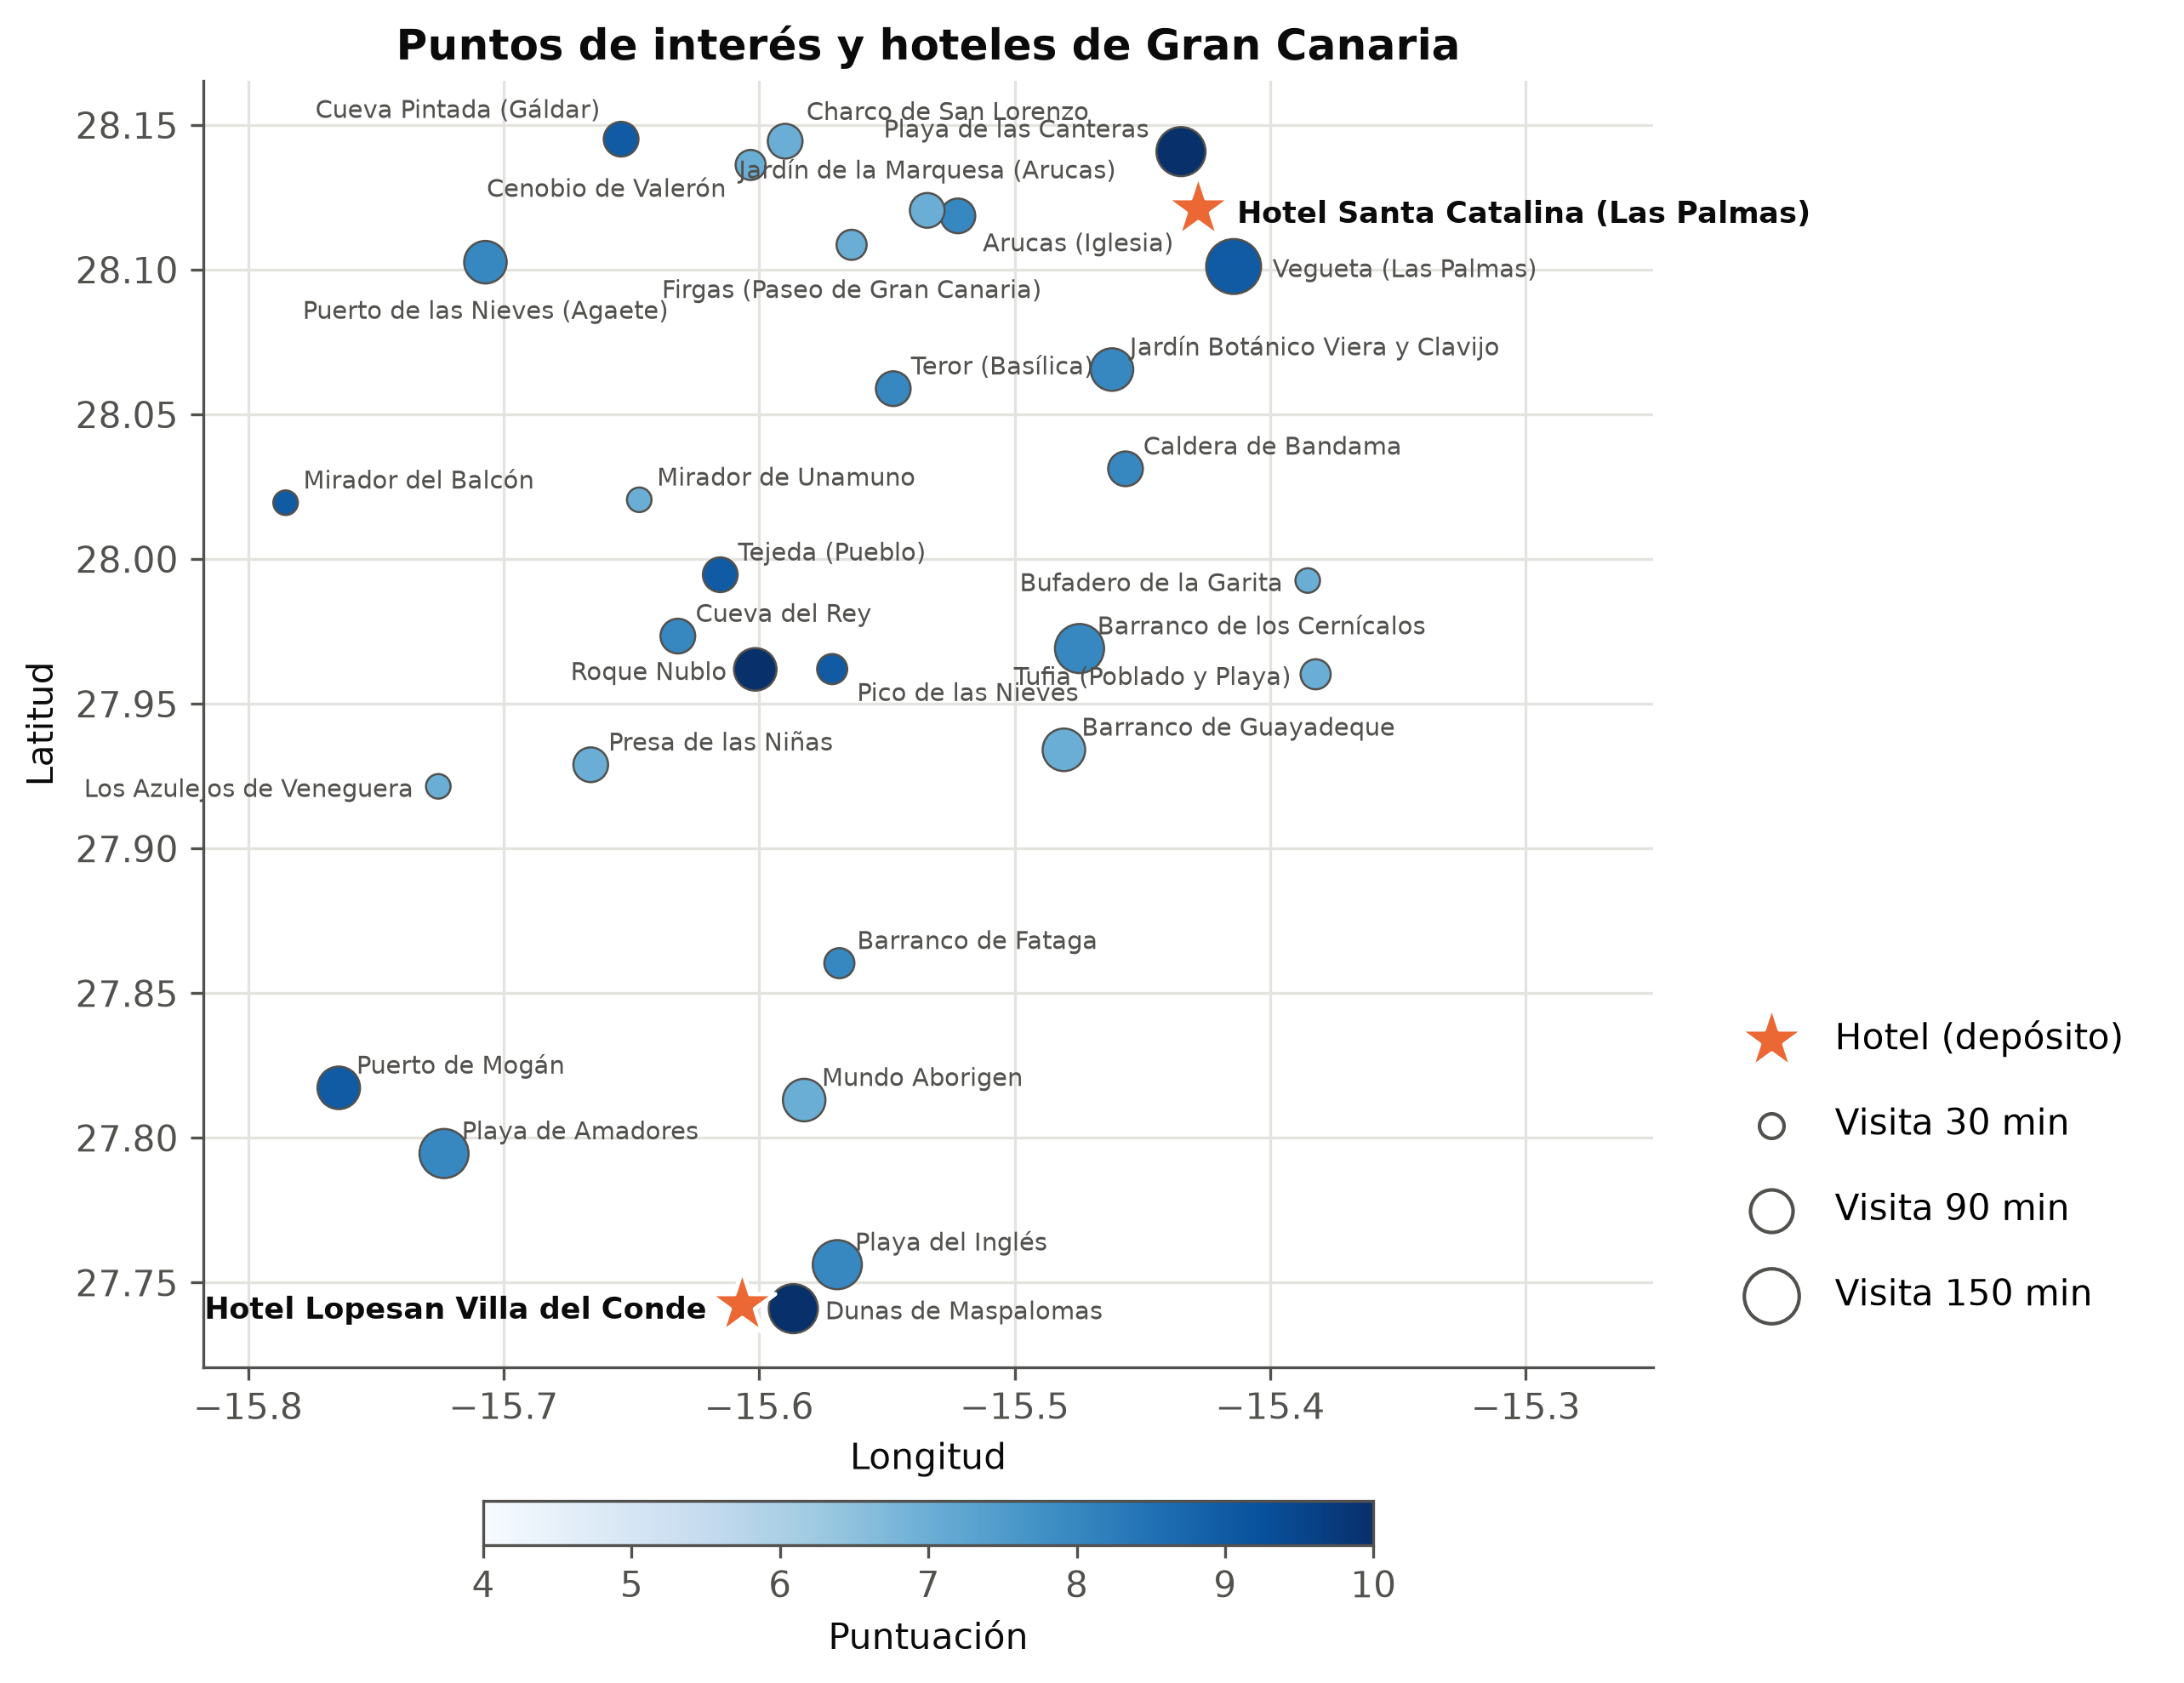
\includegraphics[width=0.72\textwidth]{mapa_pois_hoteles.png}
\caption{Puntos de interés y hoteles. El color indica la puntuación y el tamaño, el tiempo de visita.}
\label{fig:mapa}
\end{figure}

\begin{table}[H]
\centering
\small
\caption{Origen y licencia de los datos.}
\label{tab:fuentes}
\begin{tabularx}{\textwidth}{@{}l X X@{}}
\toprule
Dato & Fuente & Licencia y uso \\
\midrule
Red de carreteras & OpenStreetMap, descargada con OSMnx \citep{boeing2017} & © colaboradores de OpenStreetMap, licencia ODbL 1.0 \\
Coordenadas de los hoteles & Google Maps, consulta manual & Solo coordenadas puntuales \\
Coordenadas de los POIs & Recopiladas por el equipo y comprobadas dentro de la isla & Datos propios \\
Tiempos de referencia & Google Maps, consulta manual: 12 pares para calibrar y 4 para validar & Muestra pequeña para ajustar y comprobar; no se redistribuye \\
Puntuaciones y visitas & Propuestas con un asistente de IA, revisadas por el equipo y contrastadas con Google Maps & Valores ilustrativos propios \\
\bottomrule
\end{tabularx}
\end{table}

La matriz de tiempos deriva de OpenStreetMap, por lo que debe atribuirse y distribuirse con la misma licencia ODbL.

\paragraph{Puntuaciones.} Las puntuaciones y los tiempos de visita no proceden de una fuente medible y reflejan un criterio razonable pero subjetivo. Para contrastarlas se consultaron las valoraciones de Google Maps de 25 de los 30 POIs (los cinco restantes figuran solo como localidades o con una ficha que no corresponde al lugar). La concordancia es moderada: la correlación de Spearman entre nuestra puntuación y la nota de Google es 0,43 ($p = 0{,}032$), y la nota media sube con la puntuación (4,52 con un 7, 4,53 con un 8, 4,70 con un 9 y 4,73 con un 10). Como las notas de Google se concentran entre 4,1 y 4,8 y apenas distinguen entre lugares, se mantuvieron las puntuaciones originales. Su efecto en las rutas se estudia en la sección~\ref{sec:sensibilidad}.

\subsection{Preprocesado: construcción de la matriz de tiempos}

La matriz se genera en cinco pasos con un cuaderno ejecutable en Google Colab, \code{scripts/build\_time\_matrix.ipynb}:
\begin{enumerate}
  \item \textbf{Grafo viario.} Se descarga la red conducible de la isla y se conserva su mayor componente fuertemente conexa, de modo que desde cualquier nodo se puede llegar a cualquier otro respetando los sentidos únicos.
  \item \textbf{Velocidades.} Cada tramo recibe su velocidad máxima o, si falta, la media de su tipo de vía; con su longitud se obtiene el tiempo de recorrido.
  \item \textbf{Penalización por curvas.} A la velocidad legal, las carreteras de montaña salen demasiado rápidas. Para cada tramo se mide la curvatura $c$ (grados girados por kilómetro) y se reduce la velocidad:
  \begin{equation}
    v_{\mathrm{efectiva}} = \frac{v_{\mathrm{límite}}}{1 + c/K},
  \end{equation}
  con un mínimo de 15 km/h. $K$ se elige entre varios candidatos comparando con Google Maps, y solo se aplica si reduce el error medio al menos 0,5 min. El valor elegido fue $K = 3000$ grados/km: un tramo con 300 °/km circula un 9 \% más lento y el más sinuoso, la mitad de rápido.
  \item \textbf{Asociación a la red.} Cada POI y cada hotel se asocia al nodo de carretera más cercano.
  \item \textbf{Caminos mínimos.} Se ejecuta el algoritmo de \citet{dijkstra1959} desde cada uno de los 32 nodos y se obtiene una matriz $32 \times 32$ en minutos, sin valores infinitos.
\end{enumerate}
La matriz es asimétrica: la mayor diferencia entre $t_{ij}$ y $t_{ji}$ es de 5,2 min, por calles de sentido único y accesos distintos. Fuera de la diagonal, los tiempos van de 2,2 a 132 min, con mediana de 53,6 min. Para cada hotel se guarda un conjunto de 31 nodos con la matriz, los POIs y las coordenadas.

\subsection{Calibración y validación}

Los tiempos de OSMnx son optimistas porque suponen circulación sin tráfico, semáforos ni aparcamiento. Los 16 pares medidos en Google Maps se dividen en dos particiones: 12 pares de POIs, repartidos entre trayectos urbanos, autopista y montaña, se usan para calibrar, y 4 pares con hotel, medidos después, se reservan para validar. Tras la penalización por curvas, se aplica a toda la matriz un factor global ajustado por mínimos cuadrados por el origen sobre los pares de calibración:
\begin{equation}
  f = \frac{\sum_k m_k\, g_k}{\sum_k m_k^2} = 1{,}09,
\end{equation}
donde $m_k$ es el tiempo del modelo y $g_k$ el de Google en el par $k$. Los cocientes $g_k/m_k$ varían poco (coeficiente de variación 0,08), así que un único factor es razonable.

\begin{figure}[H]
\centering
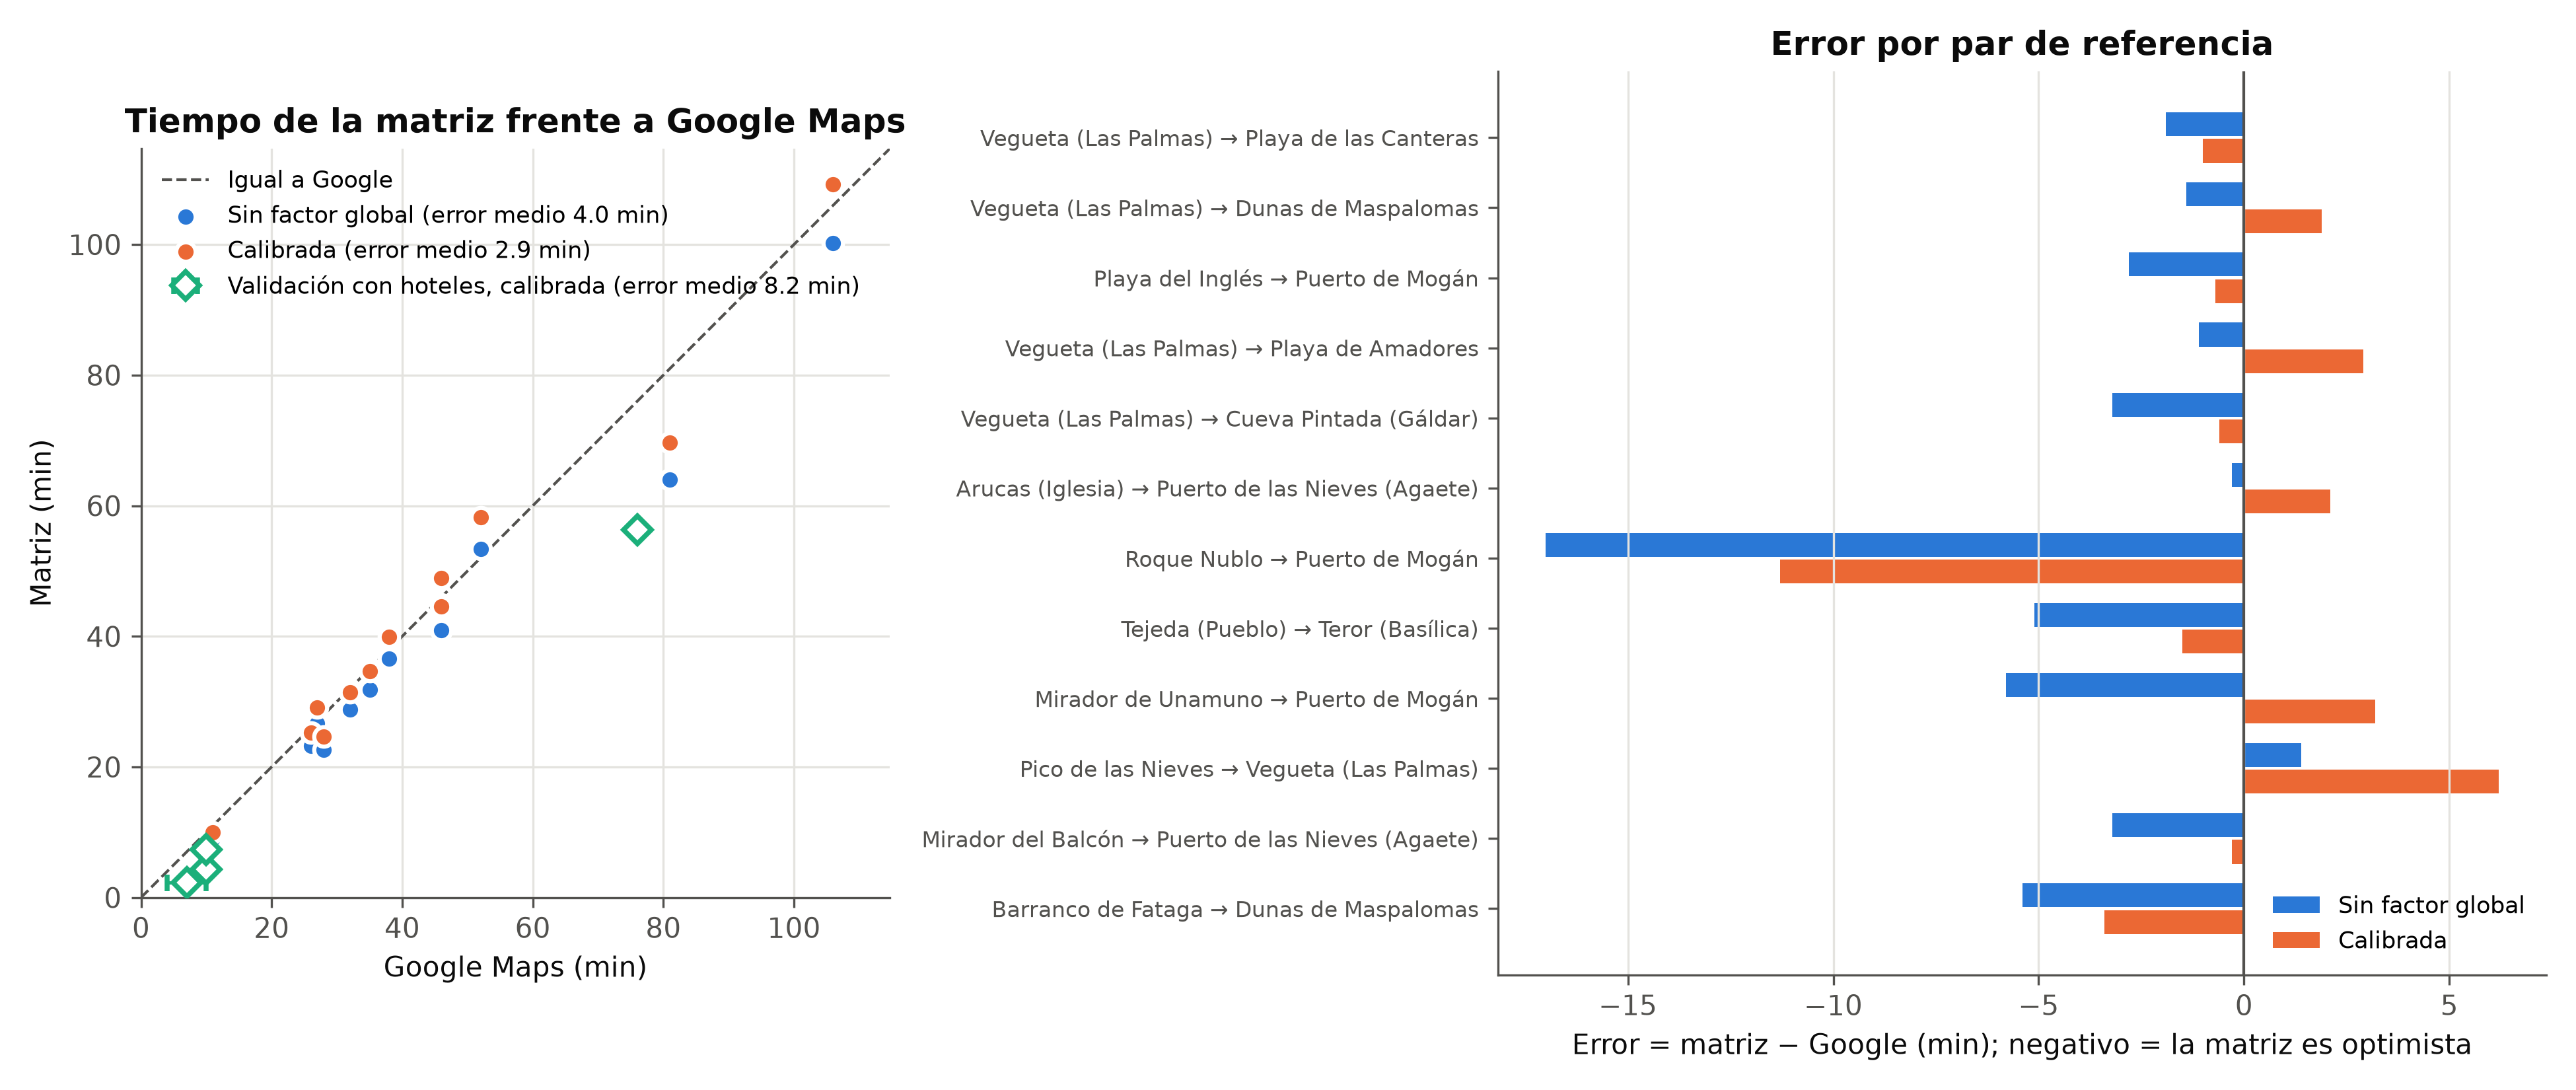
\includegraphics[width=\textwidth]{calibracion_google.png}
\caption{Calibración de la matriz frente a Google Maps: tiempos de los 12 pares de calibración y los 4 de validación (izquierda) y error por par antes y después del factor global (derecha).}
\label{fig:calibracion}
\end{figure}

\begin{table}[H]
\centering
\small
\caption{Error medio absoluto de la matriz frente a Google Maps.}
\label{tab:calibracion}
\begin{tabular}{@{}lc@{}}
\toprule
Matriz y pares evaluados & Error medio absoluto \\
\midrule
Sin factor global (con penalización por curvas), 12 pares de calibración & 4,0 min \\
Calibrada, 12 pares de calibración & 2,9 min \\
Calibrada, 4 pares de validación con hotel & 8,2 min \\
\bottomrule
\end{tabular}
\end{table}

La matriz resulta optimista en los cuatro pares de validación, y su error es casi el triple que el de calibración, lo esperable con datos que no se usaron para ajustar. Los mayores errores están en la montaña: Lopesan $\to$ Roque Nublo sale 20 min más corto que en Google (56,3 frente a 76 min). En la ciudad pesan los semáforos y el aparcamiento: Santa Catalina $\to$ Vegueta da 4,3 min frente a 10. Los tiempos deben leerse, por tanto, como estimaciones; las limitaciones se discuten en la sección~\ref{sec:limitaciones}.

\section{Experimentación y resultados}
\label{sec:experimentacion}

\subsection{Diseño experimental}

\begin{itemize}
  \item \textbf{Instancias.} Los dos hoteles, con $\Tmax = 480$ min y sin preferencias.
  \item \textbf{Presupuesto.} Todos los métodos estocásticos realizan exactamente 20.100 evaluaciones por ejecución. La heurística voraz es determinista.
  \item \textbf{Repeticiones.} 15 semillas independientes: 42, 101, 203, 314, 456, 578, 619, 723, 831, 954, 1024, 1234, 2048, 3072 y 4096.
  \item \textbf{Métricas.} Hipervolumen con punto de referencia $(\Tmax, 0) = (480\ \text{min}, 0\ \text{puntos})$ y \emph{spread} $\Delta$. Se informa de la media y de la desviación típica poblacional de las 15 ejecuciones.
  \item \textbf{Contraste.} Test pareado bilateral de rangos con signo de Wilcoxon sobre el hipervolumen de cada línea base frente a NSGA-II, con $\alpha = 0{,}05$.
\end{itemize}

\subsection{Validación en problemas de prueba}
\label{sec:zdt}

Antes de aplicarlo al caso real, el núcleo de NSGA-II (ordenación no dominada, aglomeración y torneo) se validó en tres problemas ZDT \citep{zitzler2000} con 30 variables continuas en $[0,1]$, cuyo frente es conocido. En los tres, $f_1(x) = x_1$, $g(x) = 1 + \frac{9}{29}\sum_{i=2}^{30} x_i$ y $f_2(x) = g(x)\,h(f_1, g)$, y el frente óptimo corresponde a $g(x) = 1$. Para variables continuas se usaron el cruce SBX ($\eta_c = 15$, cada variable cruzada con probabilidad 0,5) y la mutación polinomial ($\eta_m = 20$, probabilidad $1/30$ por variable), con $N = 100$, $G = 250$ y semilla 42.

\begin{table}[H]
\centering
\small
\caption{Validación de NSGA-II en la familia ZDT (IGD frente a 500 puntos del frente teórico).}
\label{tab:zdt}
\begin{tabular}{@{}l l l c c@{}}
\toprule
Problema & Frente & $h(f_1, g)$ & Soluciones & IGD \\
\midrule
ZDT1 & Convexo & $1 - \sqrt{f_1/g}$ & 100 & 0,0210 \\
ZDT2 & No convexo & $1 - (f_1/g)^2$ & 100 & 0,0547 \\
ZDT3 & Discontinuo & $1 - \sqrt{f_1/g} - (f_1/g)\sin(10\pi f_1)$ & 100 & 0,0127 \\
\bottomrule
\end{tabular}
\end{table}

\begin{figure}[H]
\centering
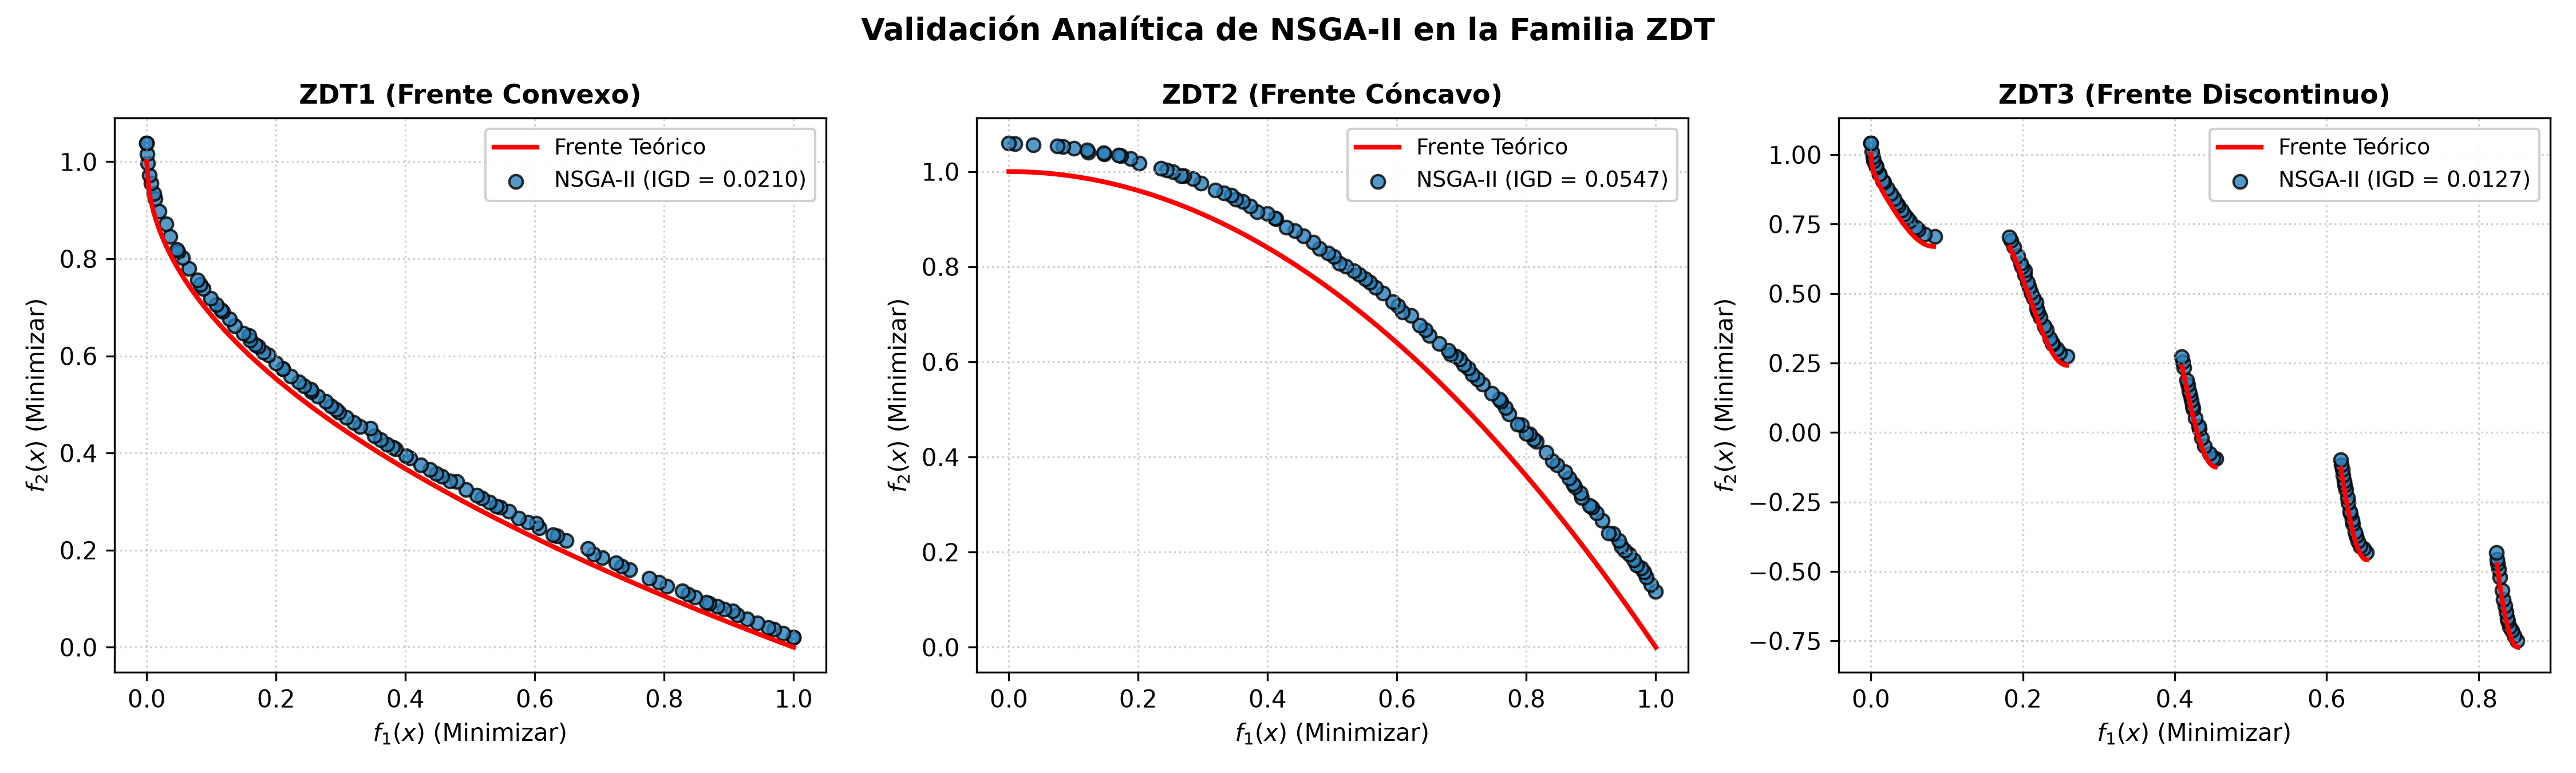
\includegraphics[width=\textwidth]{validacion_zdt_familia.png}
\caption{Frentes obtenidos por NSGA-II (puntos) frente a los frentes teóricos (línea) en ZDT1, ZDT2 y ZDT3.}
\label{fig:zdt}
\end{figure}

En los tres casos las 100 soluciones cubren todo el rango de $f_1$. En ZDT3 el algoritmo encuentra los cinco tramos del frente discontinuo y en ZDT1 queda muy cerca del frente. En ZDT2, de frente no convexo, la cobertura es completa pero las soluciones quedan algo por encima del frente teórico (figura~\ref{fig:zdt}), lo que explica su mayor IGD: con 250 generaciones la convergencia en ese problema todavía no es completa. La validación confirma que los mecanismos de dominancia y de diversidad funcionan en frentes convexos, no convexos y discontinuos.

\subsection{Comparación de algoritmos en Gran Canaria}

La tabla~\ref{tab:resultados} recoge los resultados de las 15 semillas y la figura~\ref{fig:boxplot}, su distribución.

\begin{table}[H]
\centering
\small
\caption{Hipervolumen (media $\pm$ desviación típica, 15 semillas), \emph{spread} medio y test de Wilcoxon frente a NSGA-II. La mejora es la de NSGA-II sobre cada método.}
\label{tab:resultados}
\begin{tabular}{@{}l r c c r@{}}
\toprule
Algoritmo & Hipervolumen & $\Delta$ & $p$ vs NSGA-II & Mejora \\
\midrule
\multicolumn{5}{@{}l}{\emph{Hotel Santa Catalina (Las Palmas)}} \\
NSGA-II & \textbf{11.594,3 $\pm$ 24,5} & 0,428 & --- & --- \\
Voraz & 10.188,9 $\pm$ 0,0 & 0,275 & $6{,}4 \times 10^{-4}$ & +13,8 \% \\
Búsqueda aleatoria & 10.050,3 $\pm$ 99,9 & 0,447 & $6{,}1 \times 10^{-5}$ & +15,4 \% \\
$\varepsilon$-restricción & 9.711,9 $\pm$ 254,0 & 0,307 & $6{,}1 \times 10^{-5}$ & +19,4 \% \\
Suma ponderada & 6.839,8 $\pm$ 490,3 & 1,076 & $6{,}1 \times 10^{-5}$ & +69,5 \% \\
\midrule
\multicolumn{5}{@{}l}{\emph{Hotel Lopesan Villa del Conde (Meloneras)}} \\
NSGA-II & \textbf{10.013,1 $\pm$ 64,4} & 0,597 & --- & --- \\
Voraz & 9.095,0 $\pm$ 0,0 & 0,346 & $6{,}1 \times 10^{-5}$ & +10,1 \% \\
Búsqueda aleatoria & 8.694,5 $\pm$ 90,4 & 0,632 & $6{,}1 \times 10^{-5}$ & +15,2 \% \\
$\varepsilon$-restricción & 8.389,8 $\pm$ 286,4 & 0,332 & $6{,}1 \times 10^{-5}$ & +19,3 \% \\
Suma ponderada & 5.411,4 $\pm$ 726,3 & 1,091 & $6{,}1 \times 10^{-5}$ & +85,0 \% \\
\bottomrule
\end{tabular}
\end{table}

\begin{figure}[H]
\centering
\begin{subfigure}{0.49\textwidth}
  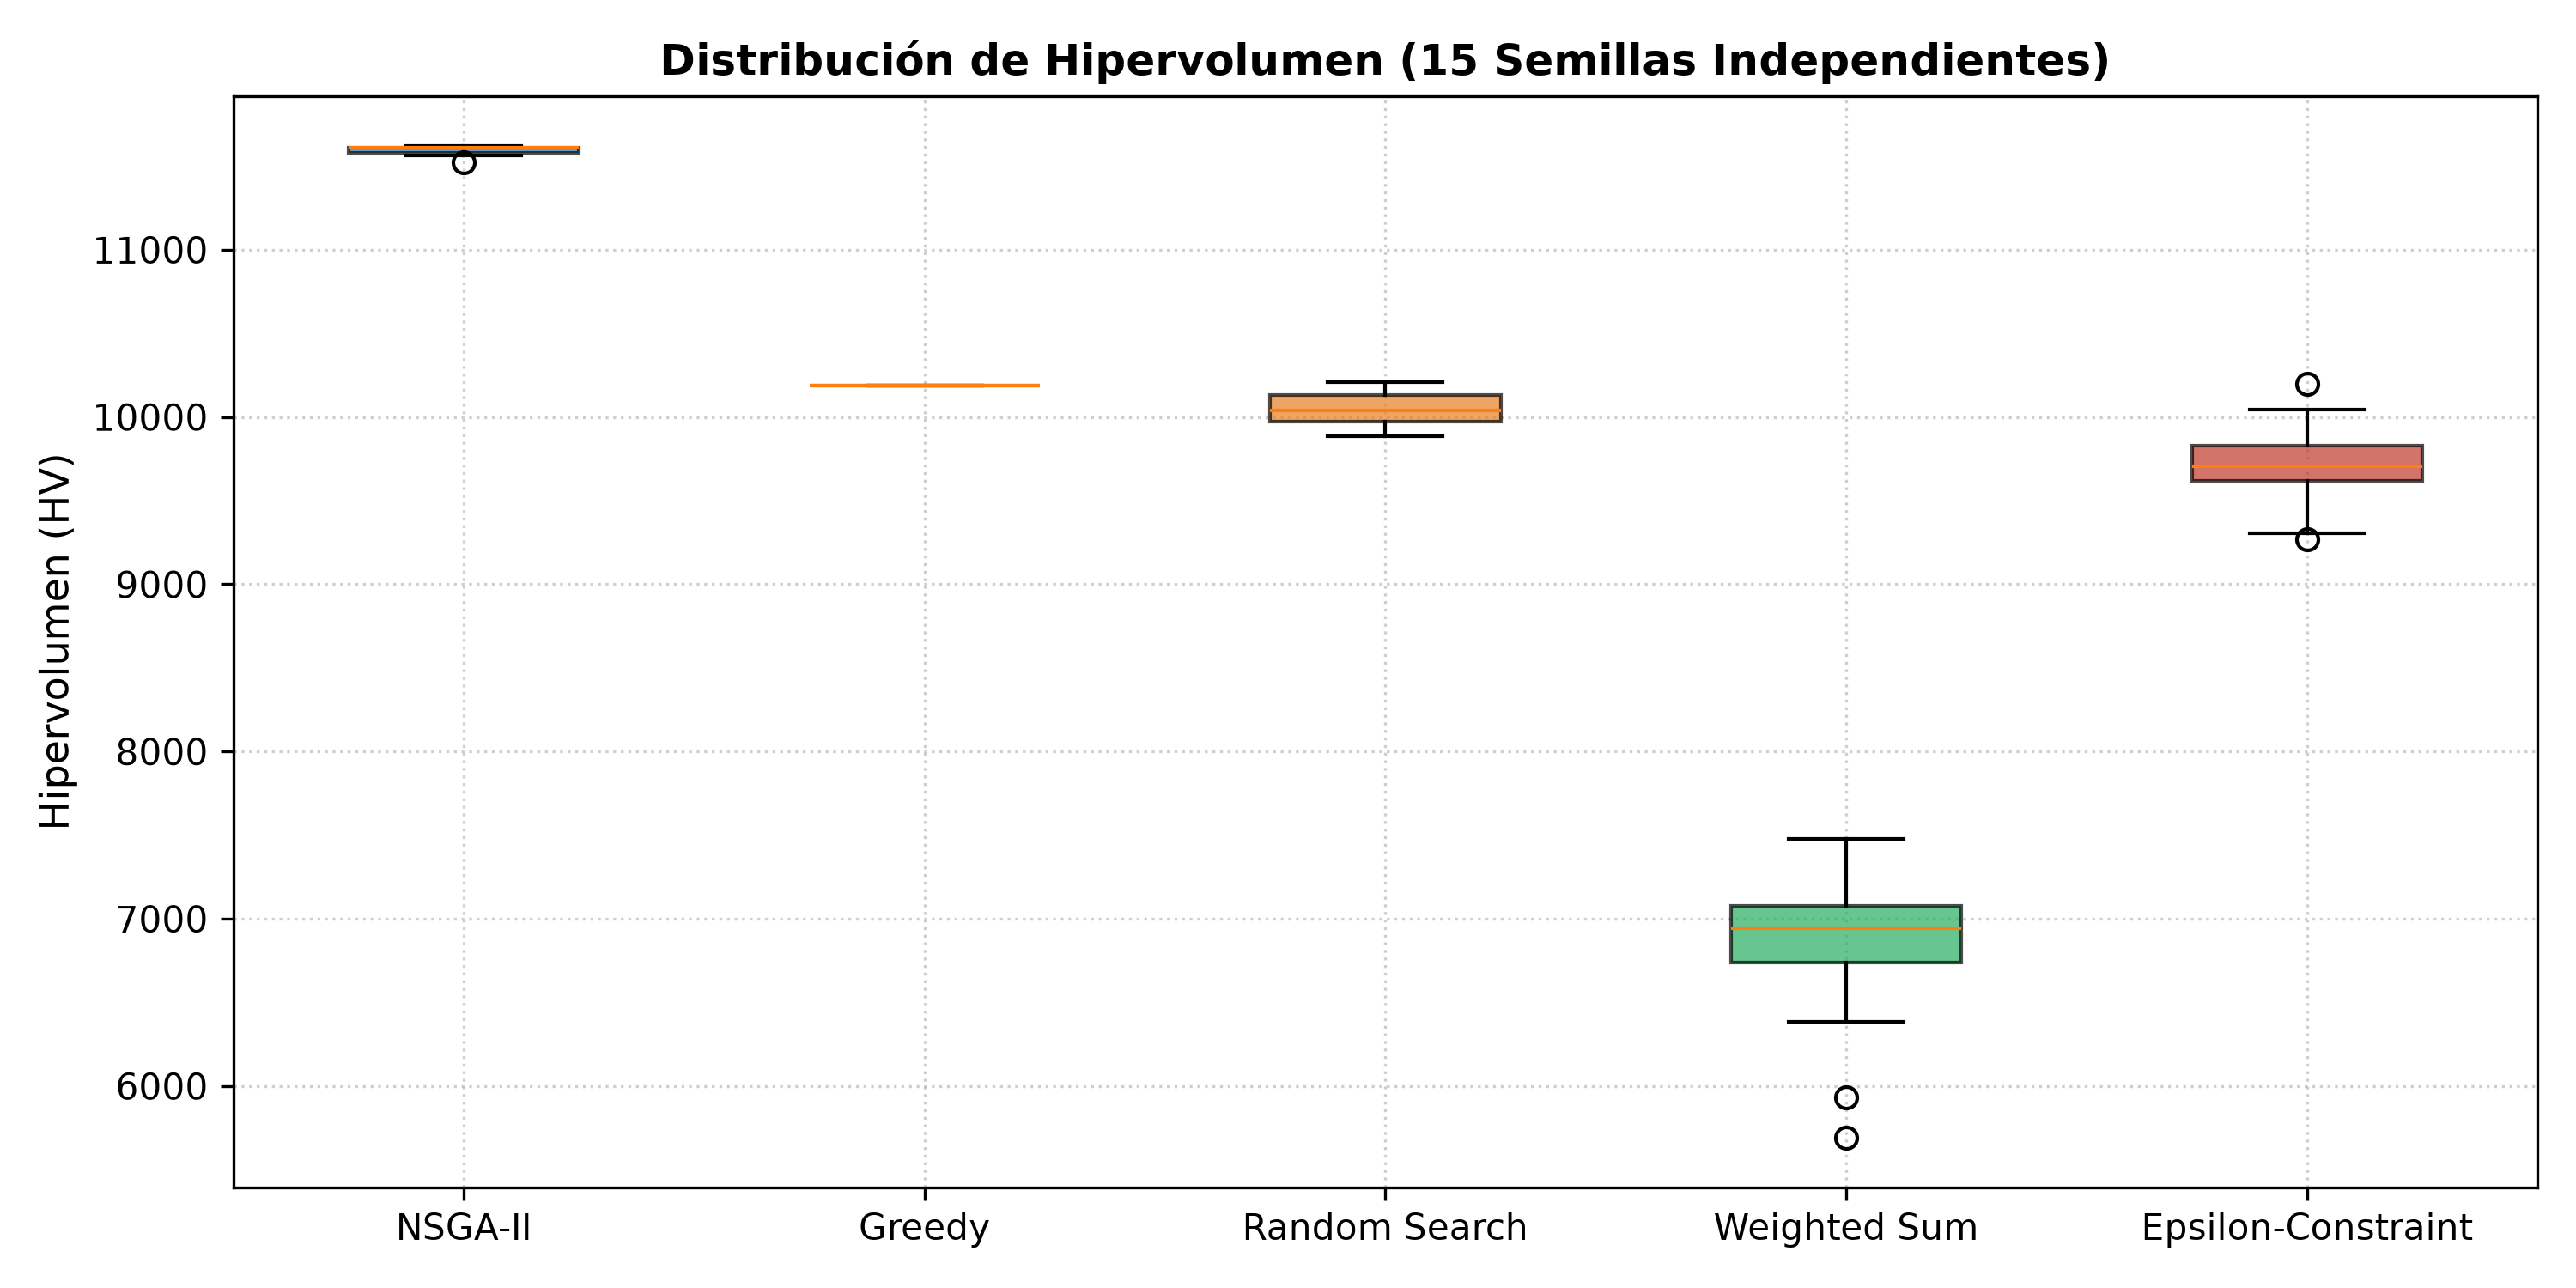
\includegraphics[width=\textwidth]{santa_catalina/boxplot_hipervolumen.png}
  \caption{Santa Catalina}
\end{subfigure}\hfill
\begin{subfigure}{0.49\textwidth}
  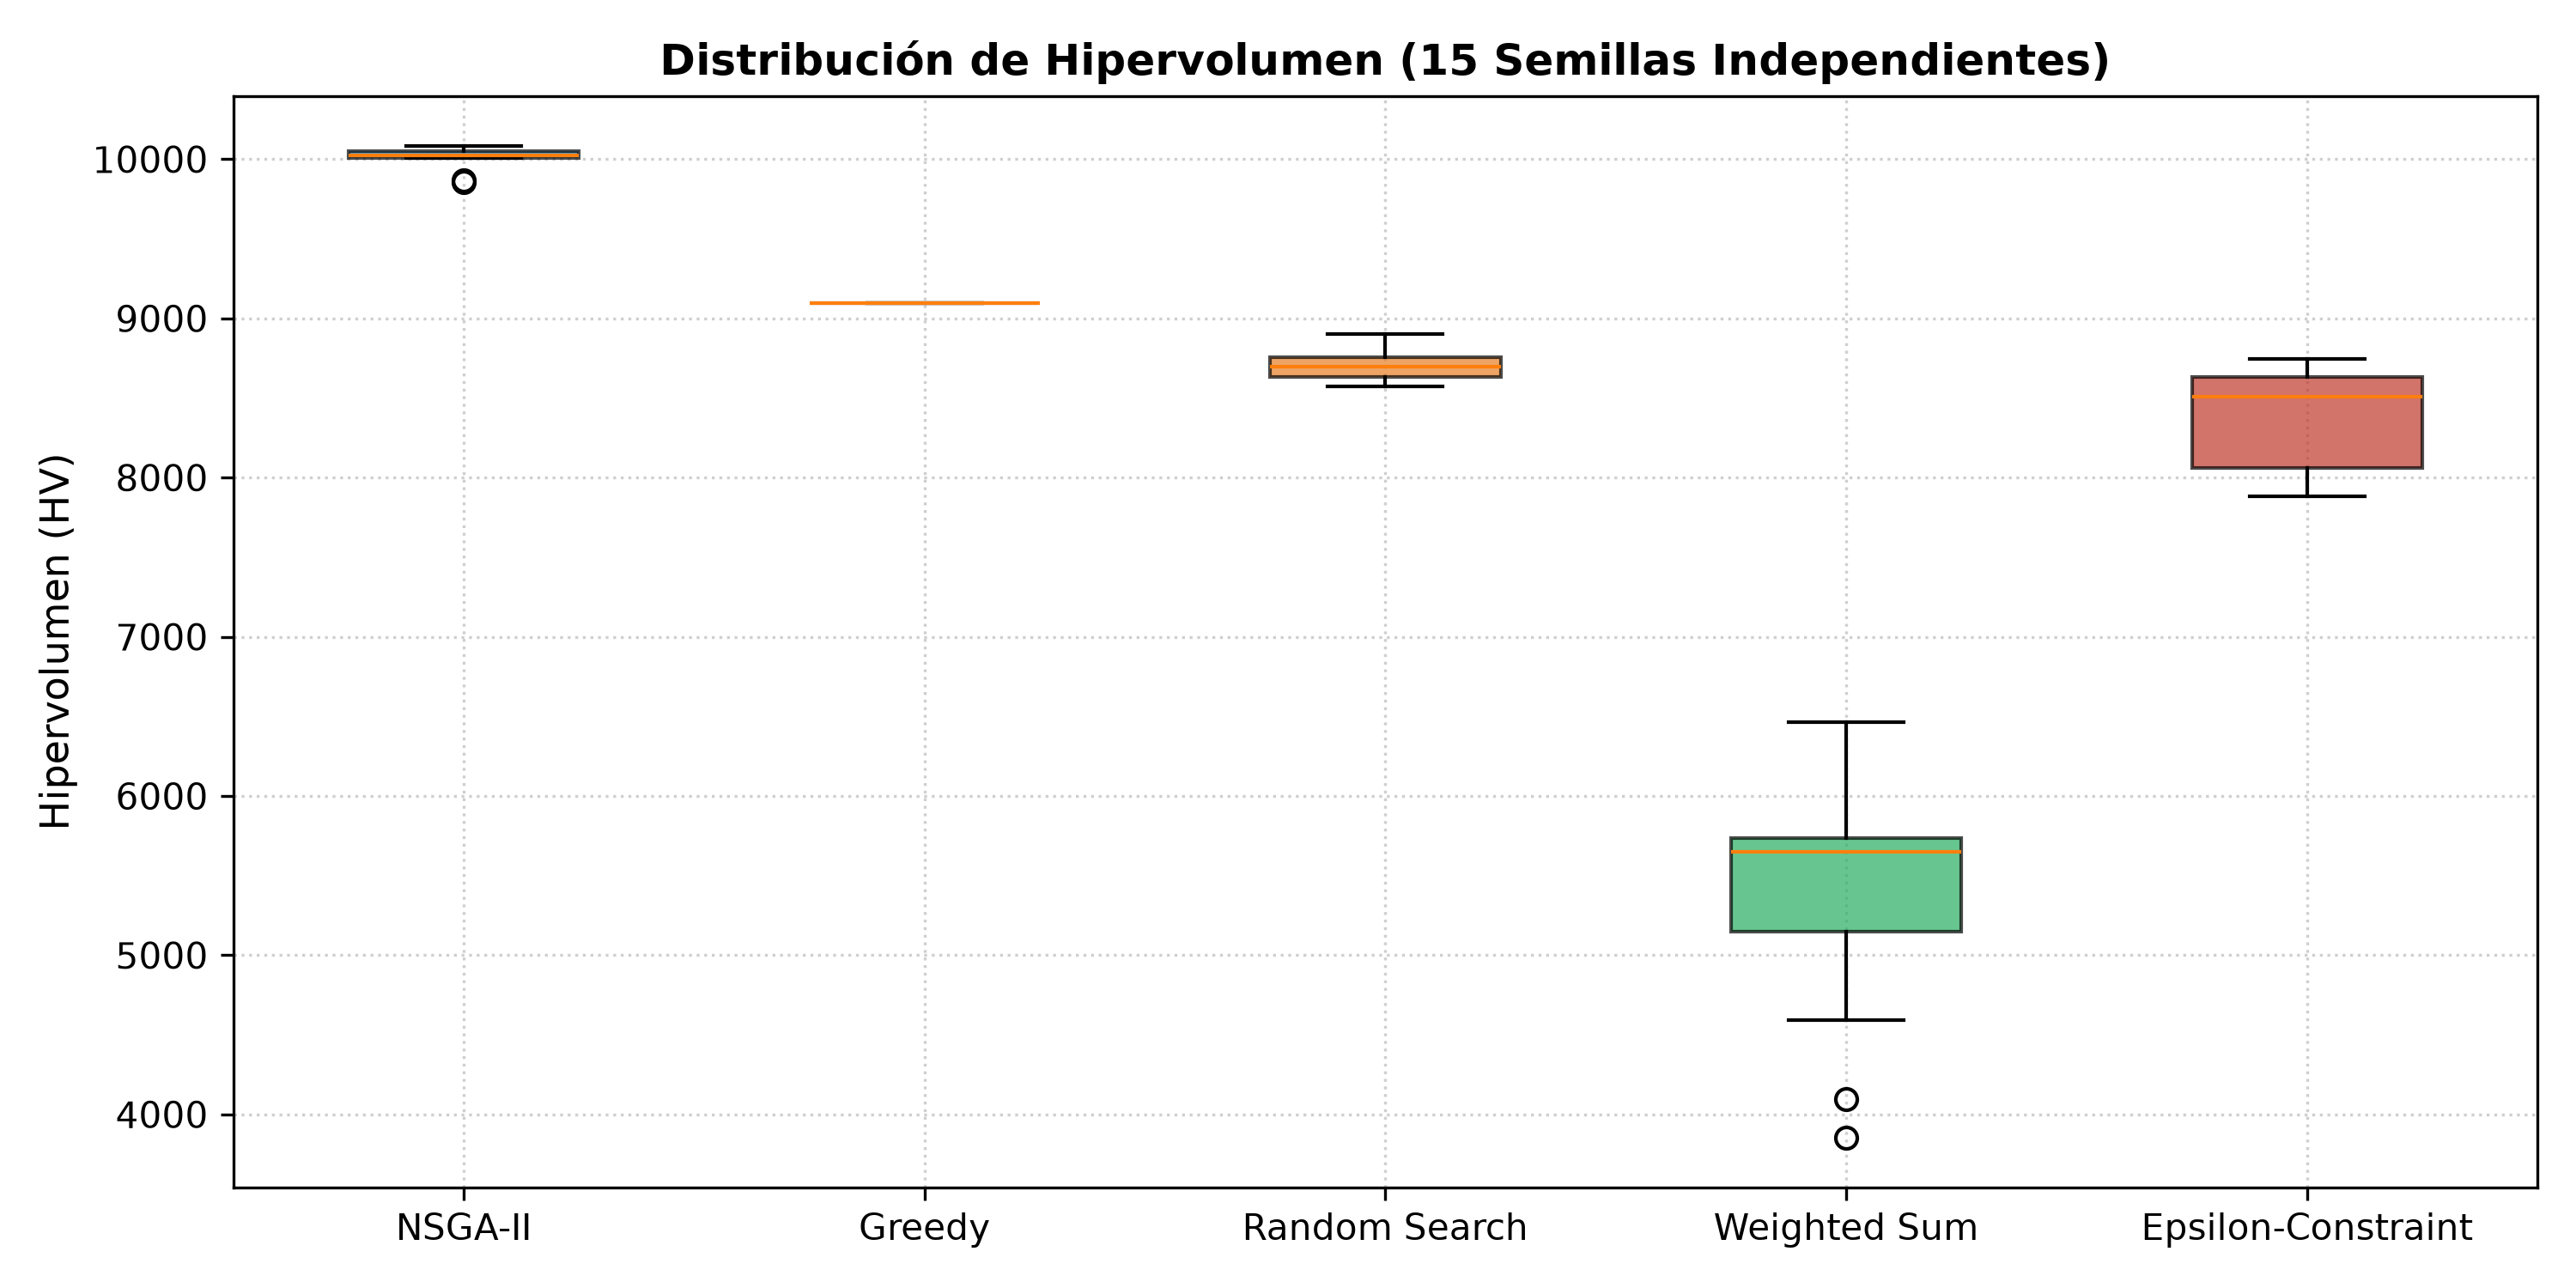
\includegraphics[width=\textwidth]{lopesan_villa_del_conde/boxplot_hipervolumen.png}
  \caption{Lopesan Villa del Conde}
\end{subfigure}
\caption{Distribución del hipervolumen de cada algoritmo en las 15 semillas.}
\label{fig:boxplot}
\end{figure}

NSGA-II obtiene el mayor hipervolumen en los dos hoteles, con diferencias significativas frente a las cuatro líneas base ($p < 0{,}001$). Gana además en las 15 semillas: su peor ejecución (11.524,5 en Santa Catalina y 9.857,0 en Lopesan) supera a la mejor de cualquier otro método. El valor $6{,}1 \times 10^{-5} = 2/2^{15}$ es el menor $p$-valor posible del test exacto de Wilcoxon con 15 pares. Frente a la heurística voraz en Santa Catalina, varias semillas de NSGA-II dan el mismo hipervolumen y la voraz es constante, así que hay empates en las diferencias y SciPy usa la aproximación normal ($p = 6{,}4 \times 10^{-4}$). La desviación típica de NSGA-II es pequeña: un 0,2 \% de la media en Santa Catalina y un 0,6 \% en Lopesan.

\paragraph{Convergencia.} La figura~\ref{fig:convergencia} muestra la evolución de una ejecución. El hipervolumen supera al de la heurística voraz en torno a la generación 10, alcanza el 99 \% de su valor final en la generación 139 y sigue mejorando despacio hasta la 200. La mejor puntuación factible avanza a saltos, cuando el algoritmo encuentra una combinación nueva de POIs que cabe en las 8 horas.

\begin{figure}[H]
\centering
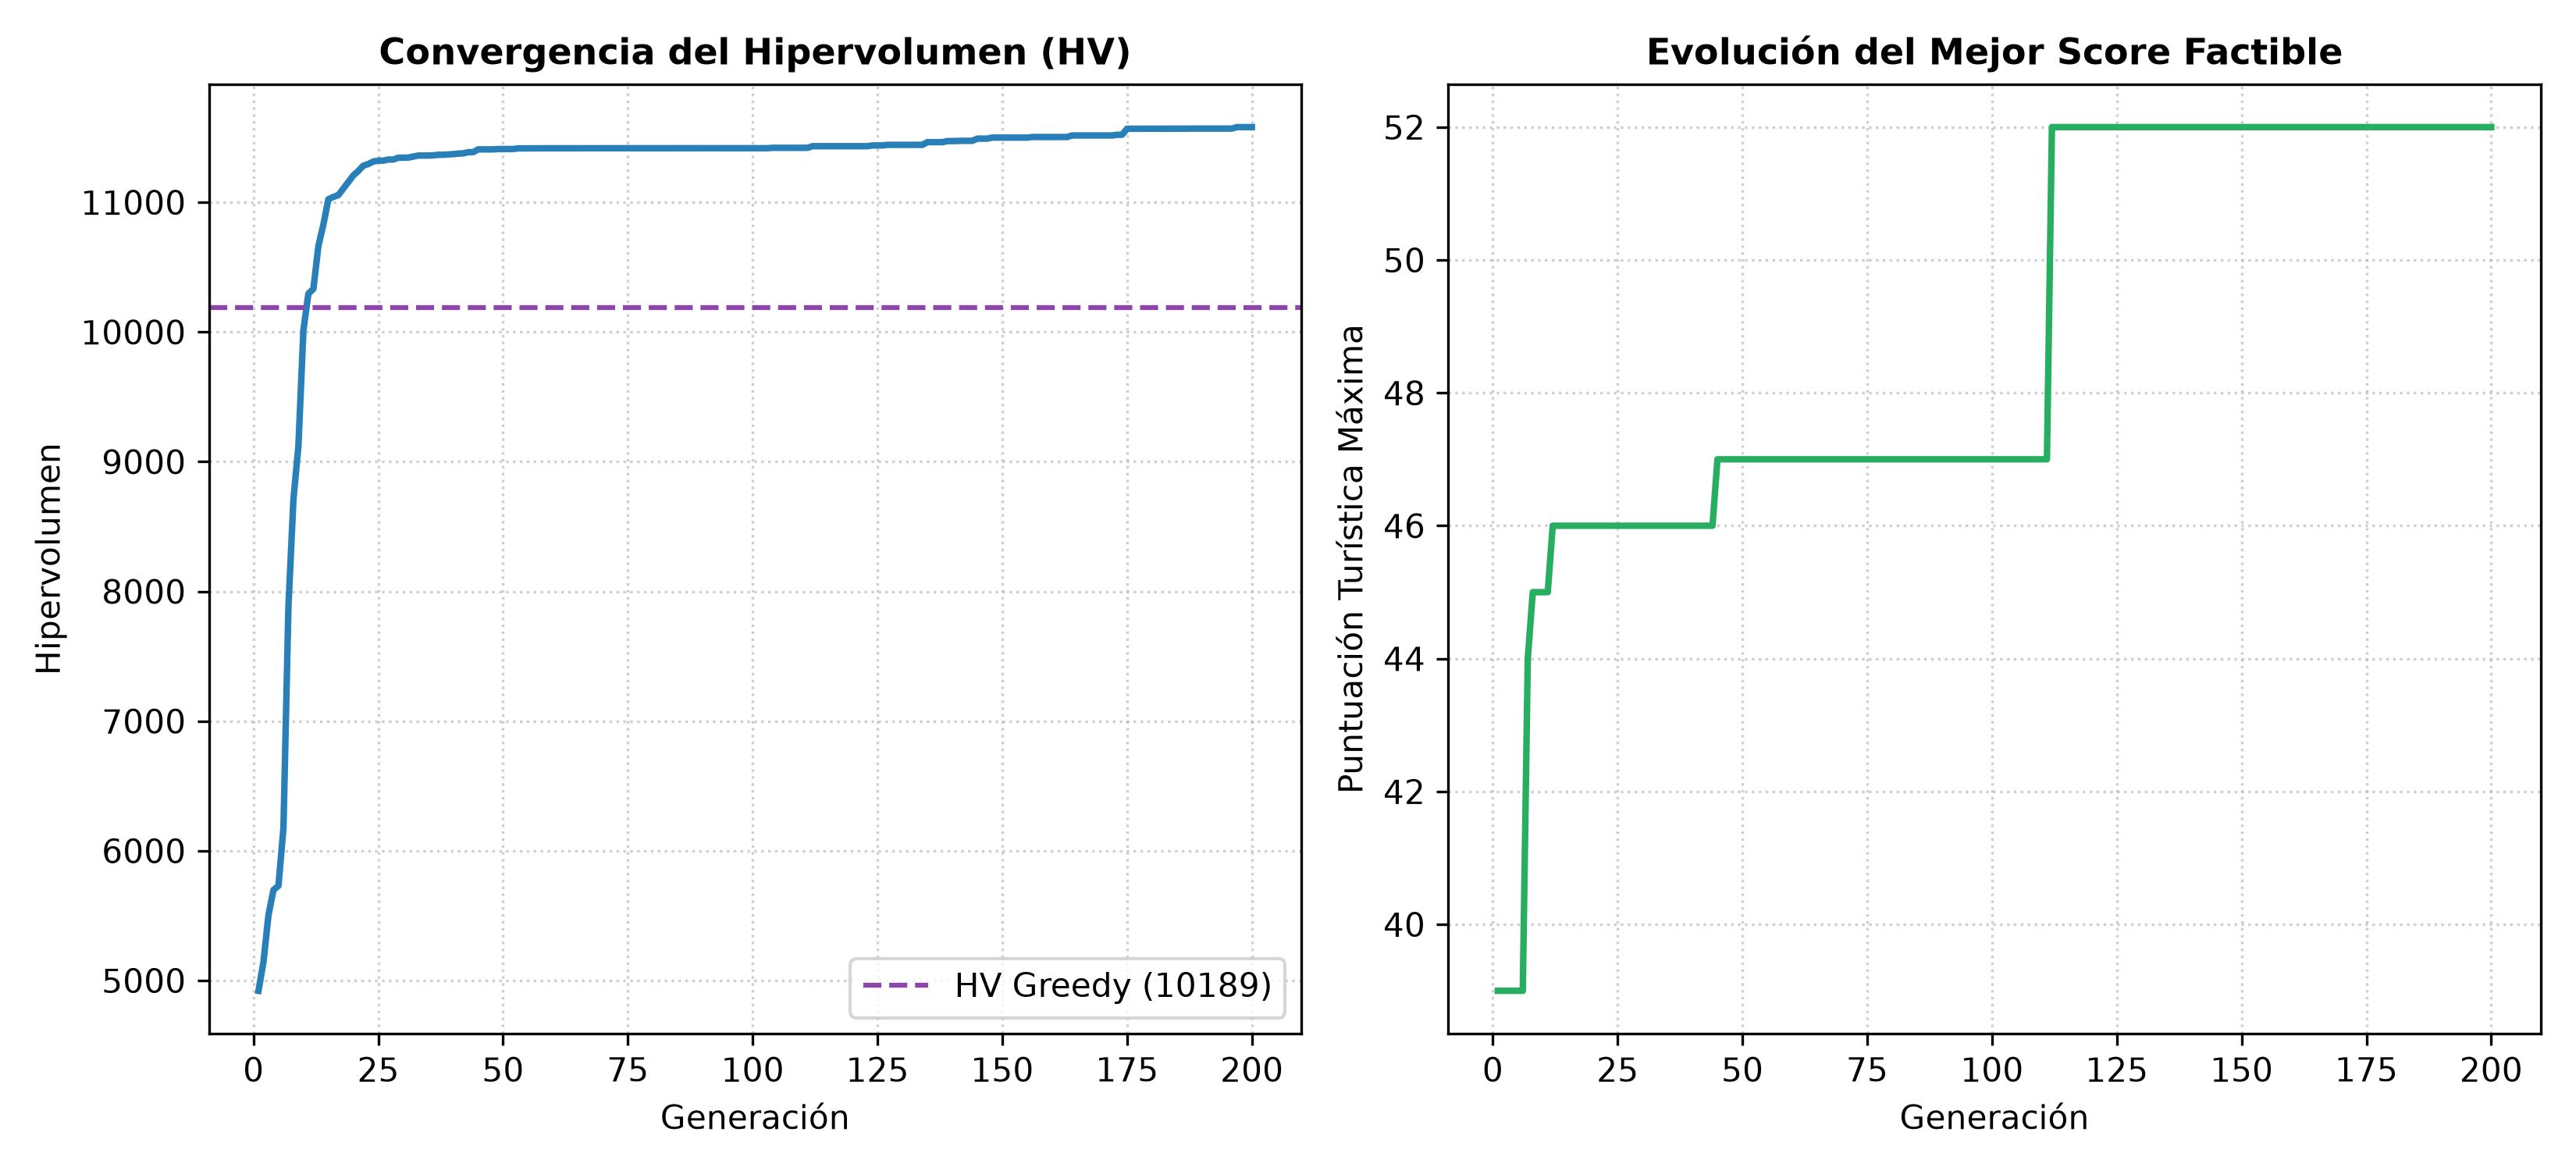
\includegraphics[width=0.9\textwidth]{santa_catalina/convergencia_nsga2.png}
\caption{Convergencia de NSGA-II en Santa Catalina (semilla 42): hipervolumen y mejor puntuación factible por generación. La línea discontinua es el hipervolumen de la heurística voraz.}
\label{fig:convergencia}
\end{figure}

\subsection{Frentes de Pareto y rutas recomendadas}

La figura~\ref{fig:frentes} muestra el frente de cada hotel con la semilla 42 y la tabla~\ref{tab:rutas}, las tres rutas recomendadas (sección~\ref{sec:recomendadas}).

\begin{figure}[H]
\centering
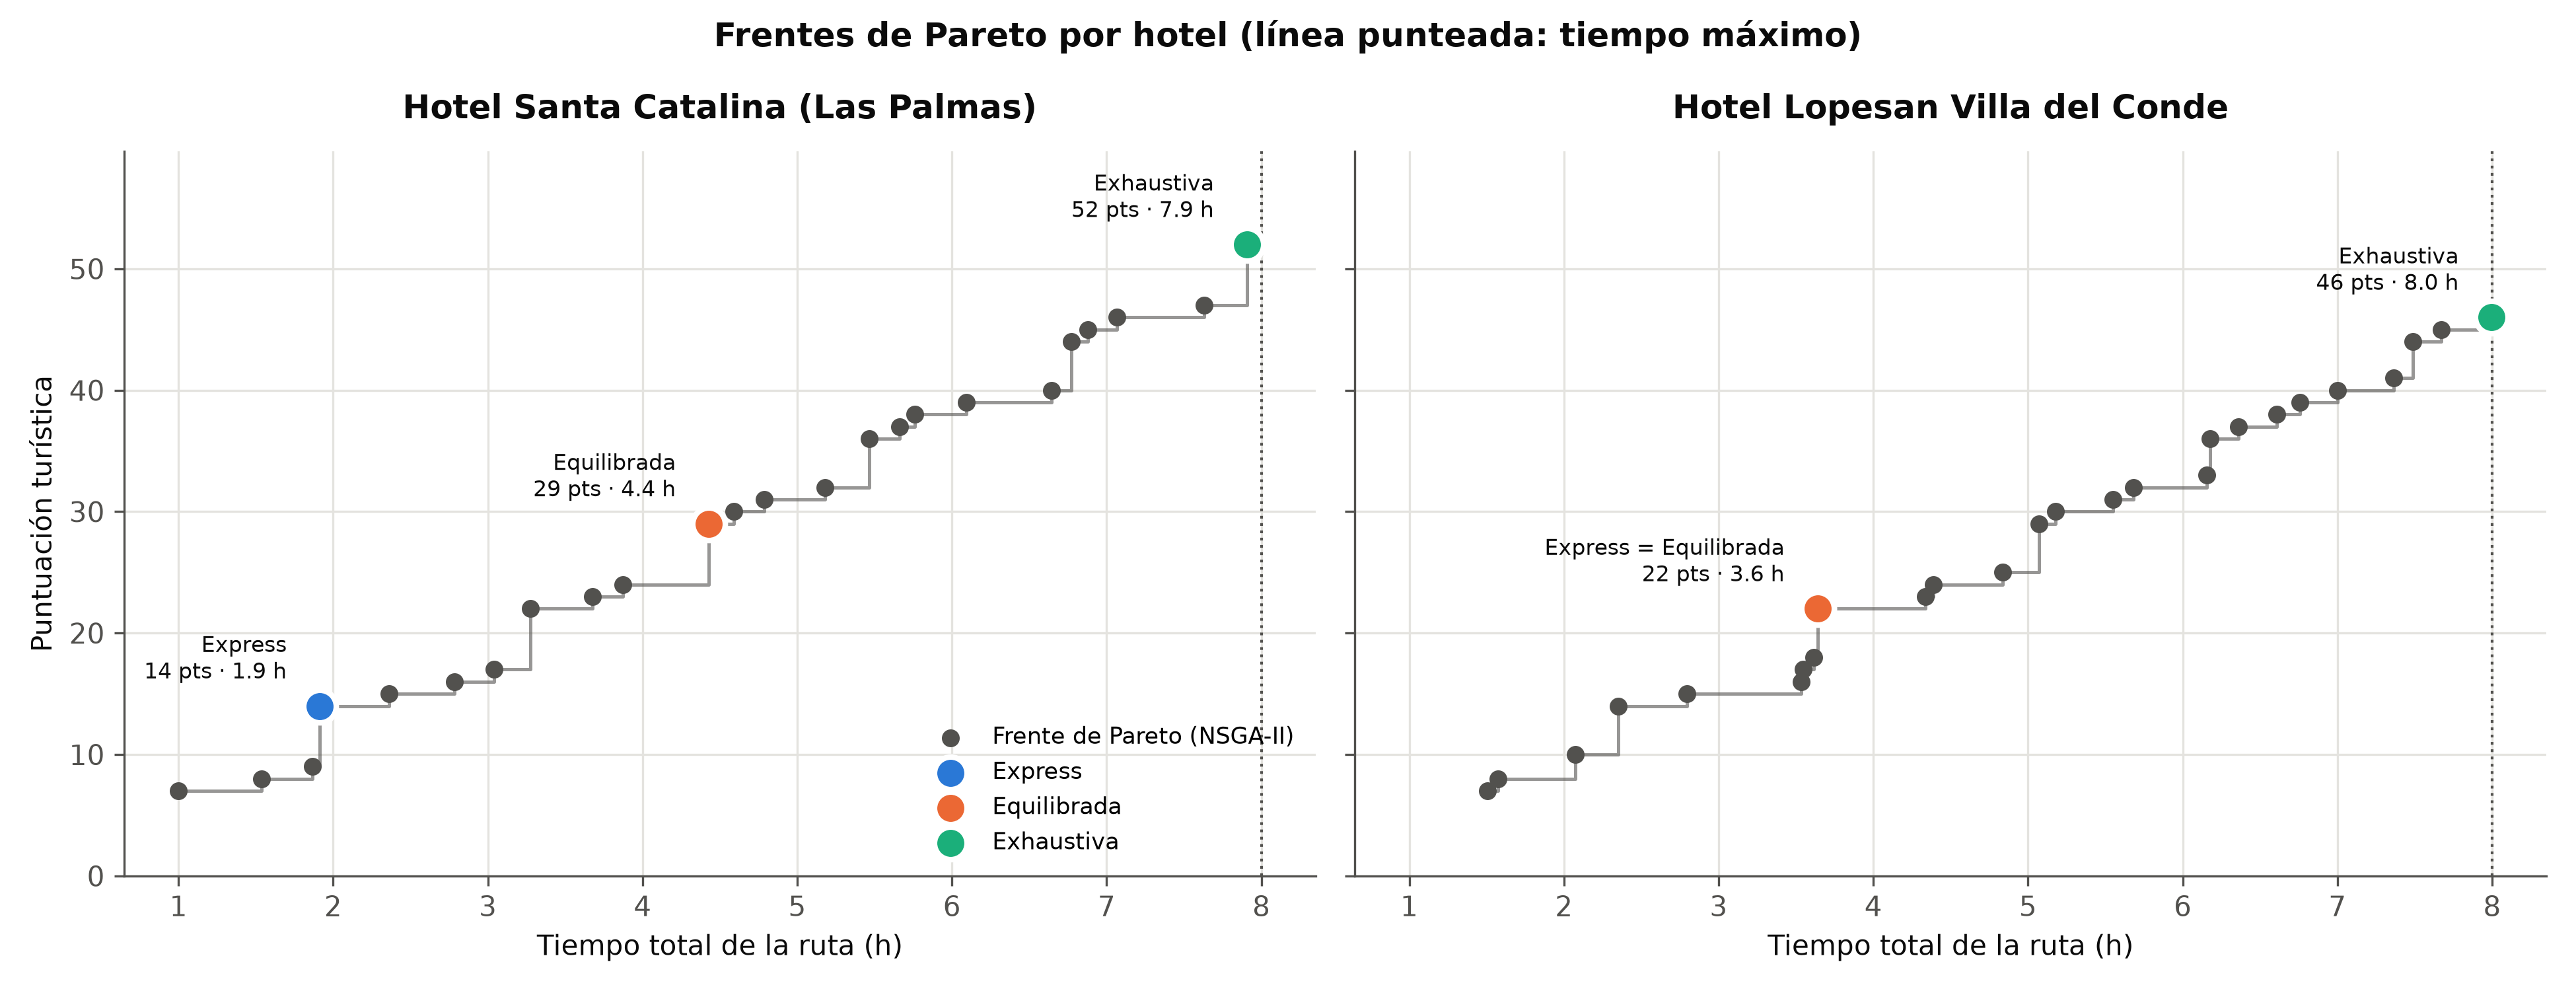
\includegraphics[width=\textwidth]{frentes_pareto.png}
\caption{Frentes de Pareto de cada hotel (semilla 42) con las rutas recomendadas. La línea punteada marca $\Tmax = 8$ h.}
\label{fig:frentes}
\end{figure}

\begin{table}[H]
\centering
\small
\caption{Rutas recomendadas (semilla 42).}
\label{tab:rutas}
\begin{tabularx}{\textwidth}{@{}l l c c X@{}}
\toprule
Hotel & Ruta & Puntos & Tiempo & Paradas \\
\midrule
Santa Catalina & Express & 14 & 1,9 h & Tufia, Bufadero de la Garita \\
 & Equilibrada & 29 & 4,4 h & Arucas, Firgas, Tufia, Bufadero \\
 & Exhaustiva & 52 & 7,9 h & Cueva Pintada, Cenobio de Valerón, Firgas, Jardín de la Marquesa, Arucas, Tufia, Bufadero \\
\midrule
Lopesan & Express y Equilibrada & 22 & 3,6 h & Tufia, Bufadero de la Garita, Barranco de Fataga \\
 & Exhaustiva & 46 & 8,0 h & Tufia, Bufadero, Cueva Pintada, Firgas, Arucas, Barranco de Fataga \\
\bottomrule
\end{tabularx}
\end{table}

Los frentes tienen unas 25 soluciones y forma escalonada: cada escalón corresponde a añadir o cambiar una parada. Desde Lopesan, la mejor ruta alcanza menos puntuación (46 frente a 52) y el hipervolumen medio es un 13,6 \% menor, porque la mayoría de los POIs están en el norte y en la cumbre. En Lopesan la ruta Express coincide con la Equilibrada: la de mejor puntuación por hora es también el punto rodilla.

\subsection{Estudio de hiperparámetros}
\label{sec:hiperparametros}

Para comprobar la configuración de la tabla~\ref{tab:parametros} se probaron, con las mismas 15 semillas y 20.100 evaluaciones:
\begin{itemize}
  \item cuatro combinaciones de población y generaciones: (50, 401), (100, 200), (150, 133) y (300, 66);
  \item una rejilla de cruce $p_c \in \{0{,}6;\ 0{,}85;\ 0{,}95\}$ por mutación $p_m \in \{0{,}15;\ 0{,}35;\ 0{,}55\}$ con $N = 100$ y $G = 200$.
\end{itemize}
Cada alternativa se compara con la configuración actual mediante el test de Wilcoxon. Como son 11 comparaciones por hotel, además del umbral 0,05 se considera el de Bonferroni, $0{,}05/11 \approx 0{,}0045$.

\begin{table}[H]
\centering
\small
\caption{Estudio de hiperparámetros: diferencia del hipervolumen medio respecto a la configuración actual ($N = 100$, $G = 200$, $p_c = 0{,}85$, $p_m = 0{,}35$) y $p$-valor de Wilcoxon.}
\label{tab:hiperparametros}
\begin{tabular}{@{}cccc rr rr@{}}
\toprule
& & & & \multicolumn{2}{c}{Santa Catalina} & \multicolumn{2}{c}{Lopesan} \\
\cmidrule(lr){5-6}\cmidrule(lr){7-8}
$N$ & $G$ & $p_c$ & $p_m$ & Dif. & $p$ & Dif. & $p$ \\
\midrule
50 & 401 & 0,85 & 0,35 & +0,03 \% & 0,733 & +0,05 \% & 0,454 \\
150 & 133 & 0,85 & 0,35 & $-$0,17 \% & 0,454 & +0,01 \% & 1,000 \\
300 & 66 & 0,85 & 0,35 & $-$0,20 \% & 0,010 & $-$0,25 \% & 0,095 \\
100 & 200 & 0,60 & 0,15 & $-$0,59 \% & $3{,}1\cdot10^{-4}$ & $-$1,00 \% & 0,010 \\
100 & 200 & 0,60 & 0,35 & $-$0,03 \% & 0,889 & $-$0,09 \% & 0,890 \\
100 & 200 & 0,60 & 0,55 & +0,09 \% & 0,041 & +0,20 \% & 0,359 \\
100 & 200 & 0,85 & 0,15 & $-$0,42 \% & 0,002 & $-$0,85 \% & 0,010 \\
100 & 200 & 0,85 & 0,55 & +0,11 \% & 0,158 & +0,34 \% & 0,073 \\
100 & 200 & 0,95 & 0,15 & $-$0,53 \% & $8{,}5\cdot10^{-4}$ & $-$0,77 \% & 0,008 \\
100 & 200 & 0,95 & 0,35 & $-$0,08 \% & 0,330 & +0,01 \% & 0,847 \\
100 & 200 & 0,95 & 0,55 & +0,06 \% & 0,530 & +0,24 \% & 0,303 \\
\bottomrule
\end{tabular}
\end{table}

Las diferencias van del $-1{,}00$ \% al $+0{,}34$ \%, de modo que la configuración elegida es razonable. El parámetro que más influye es la mutación: con $p_m = 0{,}15$ el hipervolumen baja en todos los casos, y en Santa Catalina esas caídas siguen siendo significativas con Bonferroni. Subir la mutación a 0,55 tiende a mejorar (la mayor media en los dos hoteles se obtiene con $p_c = 0{,}85$ y $p_m = 0{,}55$), pero sin significación; como la mejora se ha observado con las mismas semillas con las que se elige, habría que confirmarla con semillas nuevas antes de cambiar el valor. El cruce apenas influye. La combinación (300, 66) es la peor en los dos hoteles: con solo 66 generaciones el algoritmo no llega a converger.

\subsection{Análisis de sensibilidad}
\label{sec:sensibilidad}

Como las puntuaciones y los tiempos de visita son ilustrativos, se repitió NSGA-II (15 semillas) con cuatro variantes de los datos, manteniendo la matriz de conducción y el límite de 8 horas: visitas multiplicadas por 0,75 y por 0,5; puntuación uniforme (todos los POIs valen 8,03, la media), con la que solo cuenta el número de paradas; y puntuación cuadrática $s^2/10$, que mantiene el 10 y rebaja las puntuaciones medias, de modo que pesan más los lugares icónicos.

\begin{table}[H]
\centering
\small
\caption{Análisis de sensibilidad (medias de 15 semillas). El hipervolumen de las variantes de puntuación no es comparable con el de la base porque cambia la escala.}
\label{tab:sensibilidad}
\begin{tabular}{@{}l l r c c@{}}
\toprule
Hotel & Variante & Hipervolumen & Soluciones & Paradas (ruta más completa) \\
\midrule
Santa Catalina & Base & 11.594,3 & 24,6 & 6,9 \\
 & Visitas $\times 0{,}75$ & 14.329,8 & 30,2 & 8,0 \\
 & Visitas $\times 0{,}5$ & 18.815,0 & 43,8 & 10,0 \\
 & Uniforme & 12.166,5 & 6,3 & 6,3 \\
 & Cuadrática & 8.998,2 & 53,8 & 6,0 \\
\midrule
Lopesan & Base & 10.013,1 & 23,6 & 6,0 \\
 & Visitas $\times 0{,}75$ & 12.261,1 & 27,3 & 7,0 \\
 & Visitas $\times 0{,}5$ & 16.064,1 & 40,1 & 9,0 \\
 & Uniforme & 10.478,2 & 5,9 & 5,9 \\
 & Cuadrática & 7.941,0 & 25,1 & 5,2 \\
\bottomrule
\end{tabular}
\end{table}

Acortar las visitas a la mitad aumenta el hipervolumen un 62 \% en Santa Catalina y un 60 \% en Lopesan, y la ruta más completa pasa de 6--7 paradas a 9--10. Con puntuación uniforme el frente se reduce a unas 6 soluciones, una por número de paradas, porque entre dos rutas con las mismas paradas solo sobrevive la más corta.

Más revelador es qué POIs aparecen. En todas las variantes y en los dos hoteles, el Bufadero de la Garita, Tufia y Arucas forman el núcleo de las rutas: son visitas cortas en el noreste, junto a la autopista GC-1. En cambio, las Dunas de Maspalomas y el Roque Nublo, con la máxima puntuación, casi nunca aparecen. La tabla~\ref{tab:iconos} explica por qué: ir, visitarlos y volver cuesta más de tres horas por 10 puntos, mientras que la ruta Express de Santa Catalina da 14 puntos en 1,9 horas.

\begin{table}[H]
\centering
\small
\caption{Tiempo de ir, visitar y volver ($t_{hi} + v_i + t_{ih}$, en minutos) para los dos lugares de puntuación 10 menos elegidos.}
\label{tab:iconos}
\begin{tabular}{@{}l c c@{}}
\toprule
Desde & Dunas de Maspalomas & Roque Nublo \\
\midrule
Santa Catalina & $42{,}2 + 120 + 42{,}7 = 205{,}0$ & $69{,}2 + 90 + 70{,}8 = 230{,}0$ \\
Lopesan & $2{,}3 + 120 + 2{,}2 = 124{,}4$ & $56{,}3 + 90 + 55{,}5 = 201{,}8$ \\
\bottomrule
\end{tabular}
\end{table}

Desde Santa Catalina ninguno de los dos aparece en ninguna variante. Desde Lopesan las Dunas sí están en el 28,5 \% de las soluciones del frente, pero solo en rutas cortas, y entran en las rutas recomendadas en cuanto la visita se acorta o el 10 pesa más. El Roque Nublo solo gana presencia con la puntuación cuadrática (del 1,4 \% al 19,4 \% de las soluciones desde Lopesan); acortar la visita no basta, porque lo que pesa es la conducción de ida y vuelta, casi dos horas.

\section{Discusión}
\label{sec:discusion}

\subsection{Qué método funciona mejor y por qué}

\paragraph{NSGA-II.} Es el mejor método en los dos hoteles y en todas las semillas. Su ventaja procede de aproximar todo el frente a la vez: la población reparte el presupuesto entre todas las zonas de compromiso, la aglomeración mantiene soluciones repartidas y el elitismo conserva las mejores rutas encontradas. Los métodos de escalarización, en cambio, dividen el presupuesto en diez búsquedas aisladas de 2.010 evaluaciones cada una.

\paragraph{Suma ponderada frente a $\varepsilon$-restricción.} La comparación confirma la teoría de la escalarización. La $\varepsilon$-restricción obtiene un 42 \% más de hipervolumen que la suma ponderada en Santa Catalina y un 55 \% más en Lopesan, y reduce el \emph{spread} de 1,08 a 0,31--0,33. La suma ponderada solo puede encontrar puntos de la envoltura convexa del frente; además, sus diez pesos convergen a menudo a las mismas rutas, de modo que aporta solo entre 3 y 5 soluciones distintas. Las cotas equiespaciadas de la $\varepsilon$-restricción, en cambio, reparten las soluciones a lo largo del eje del tiempo y alcanzan también las zonas no convexas.

\paragraph{La $\varepsilon$-restricción, por debajo de las heurísticas simples.} Aun así, la $\varepsilon$-restricción queda por debajo de la heurística voraz y de la búsqueda aleatoria en los dos hoteles (9.712 frente a 10.189 y 10.050 en Santa Catalina; 8.390 frente a 9.095 y 8.695 en Lopesan). La causa es estructural: con 10 cotas, su frente tiene como mucho 10 puntos, mientras que la voraz prueba 29 presupuestos y la búsqueda aleatoria conserva todas las rutas no dominadas de sus 20.100 muestras. Como el hipervolumen de un frente escalonado crece con el número de escalones, un método con pocos puntos queda penalizado aunque cada punto sea bueno. Una rejilla más fina mejoraría su cobertura, pero repartiría aún más el presupuesto. Esto muestra que, con un presupuesto fijo, la forma de repartirlo importa tanto como la calidad de cada subproblema.

\paragraph{La heurística voraz.} Es la mejor línea base, aunque no está sujeta al mismo presupuesto: es determinista y construye cada ruta en una sola pasada, sin evaluar soluciones completas. Su buen resultado indica que la regla de puntuación por minuto captura bien la estructura del problema, lo que coincide con el análisis de sensibilidad. NSGA-II la supera entre un 10 \% y un 14 \% porque puede reordenar las paradas y combinar lugares que la regla voraz descarta en los primeros pasos.

\paragraph{Validación ZDT.} En ZDT1 y ZDT3 el frente obtenido queda muy cerca del teórico. En ZDT2 la cobertura es completa pero la convergencia no, lo que indica que en problemas continuos no convexos harían falta más generaciones. No afecta al caso real, en el que la convergencia se ha comprobado directamente.

\subsection{Influencia de los datos}

Las rutas dependen sobre todo de la puntuación por minuto de cada lugar, no de su puntuación. Por eso el núcleo de las rutas lo forman visitas cortas y cercanas a la autopista (Bufadero de la Garita, Tufia, Arucas), y los iconos de la isla (las Dunas, el Roque Nublo) solo aparecen si se acortan las visitas o se premian los lugares de máxima puntuación. La ubicación del hotel también pesa: desde el sur el frente pierde un 13,6 \% de hipervolumen porque la mayoría de los POIs están en el norte. Si se quiere que las rutas incluyan los iconos, la decisión depende del perfil de turista: cambiar la escala de puntuación o marcarlos como visita obligatoria, que el modelo ya admite.

\subsection{Limitaciones}
\label{sec:limitaciones}

\begin{itemize}
  \item \textbf{Tiempos aproximados.} La matriz es optimista: el error de validación es de 8,2 min y en la montaña llega a 20 min. No se modela el tráfico, el aparcamiento ni la variación horaria. Un único factor global no basta para las carreteras de la cumbre; factores por tipo de trayecto o una fuente de tiempos con tráfico mejorarían la precisión.
  \item \textbf{Puntuaciones subjetivas.} Las puntuaciones y los tiempos de visita son ilustrativos. Concuerdan moderadamente con Google Maps, pero otro criterio cambiaría las rutas, como muestra el análisis de sensibilidad.
  \item \textbf{Modelo simplificado.} No se consideran horarios de apertura, ventanas de tiempo, el tiempo de comida ni rutas de varios días. Algunos POIs quedan lejos de la carretera y su tiempo de conducción llega solo al nodo de red más cercano. La red refleja los cortes de carretera en el momento de la descarga.
  \item \textbf{Frente aproximado.} No se ha calculado el frente exacto del caso real, por lo que no puede medirse cuánto le falta a NSGA-II para alcanzarlo; solo se sabe que supera a las líneas base. El modelo entero de la sección~\ref{sec:formulacion} permitiría calcularlo con un resolvedor.
  \item \textbf{Elección de parámetros.} Los hiperparámetros se evaluaron con las mismas 15 semillas de la comparación, así que pequeñas mejoras, como la de subir la mutación, deben confirmarse con semillas nuevas.
\end{itemize}

\section{Conclusiones y trabajo futuro}
\label{sec:conclusiones}

Se ha planteado la planificación de una ruta turística de un día en Gran Canaria como un problema de orientación biobjetivo y se ha resuelto con una implementación propia de NSGA-II sobre datos reales. Las principales conclusiones son:

\begin{itemize}
  \item Es posible construir una matriz de tiempos realista con OpenStreetMap: con una penalización por curvas y un factor calibrado, el error frente a Google Maps es de 2,9 min en los pares de calibración, aunque sube a 8,2 min fuera de muestra y la montaña sigue siendo el caso más difícil.
  \item El problema admite una formulación entera clara y una representación por secuencias equivalente, en la que solo la restricción de tiempo debe tratarse durante la búsqueda. Las preferencias del turista se integran como restricciones con una condición de factibilidad sencilla y se garantizan con un operador de reparación.
  \item NSGA-II supera a la heurística voraz, a la búsqueda aleatoria, a la suma ponderada y a la $\varepsilon$-restricción en los dos hoteles y en todas las semillas, con el mismo presupuesto y diferencias significativas. La $\varepsilon$-restricción mejora claramente a la suma ponderada, como predice la teoría, pero dividir el presupuesto en pocos subproblemas la deja por debajo de las heurísticas simples.
  \item La configuración de NSGA-II es razonable; la mutación es el parámetro que más influye.
  \item Las rutas óptimas dependen sobre todo de la puntuación por minuto de cada lugar y de la posición del hotel. Los lugares de visita larga o alejados solo entran si cambia la valoración, lo que hay que tener en cuenta al usar el modelo con turistas reales.
\end{itemize}

\paragraph{Trabajo futuro.} Las extensiones más naturales son: calcular el frente exacto con el modelo entero para medir la calidad de NSGA-II; usar tiempos con tráfico o factores de calibración por tipo de vía; añadir horarios de apertura (OP con ventanas de tiempo) y rutas de varios días (Team OP); obtener las puntuaciones de fuentes medibles, como reseñas o encuestas; considerar varias visitas obligatorias; y comparar con otros algoritmos evolutivos multiobjetivo.


\begin{thebibliography}{99}
\addcontentsline{toc}{section}{Referencias}
\small

\bibitem[Audet et~al.(2021)]{audet2021}
Audet, C., Bigeon, J., Cartier, D., Le~Digabel, S. y Salomon, L. (2021).
\newblock Performance indicators in multiobjective optimization.
\newblock \emph{European Journal of Operational Research}, 292(2), 397--422.

\bibitem[Bérubé et~al.(2009)]{berube2009}
Bérubé, J.-F., Gendreau, M. y Potvin, J.-Y. (2009).
\newblock An exact $\varepsilon$-constraint method for bi-objective combinatorial optimization problems: Application to the Traveling Salesman Problem with Profits.
\newblock \emph{European Journal of Operational Research}, 194(1), 39--50.
\newblock \url{https://doi.org/10.1016/j.ejor.2007.12.014}

\bibitem[Boeing(2017)]{boeing2017}
Boeing, G. (2017).
\newblock OSMnx: New methods for acquiring, constructing, analyzing, and visualizing complex street networks.
\newblock \emph{Computers, Environment and Urban Systems}, 65, 126--139.
\newblock \url{https://doi.org/10.1016/j.compenvurbsys.2017.05.004}

\bibitem[Coello~Coello et~al.(2007)]{coello2007}
Coello~Coello, C.~A., Lamont, G.~B. y Van~Veldhuizen, D.~A. (2007).
\newblock \emph{Evolutionary Algorithms for Solving Multi-Objective Problems} (2.ª ed.).
\newblock Springer.

\bibitem[Das y Dennis(1997)]{dasdennis1997}
Das, I. y Dennis, J.~E. (1997).
\newblock A closer look at drawbacks of minimizing weighted sums of objectives for Pareto set generation in multicriteria optimization problems.
\newblock \emph{Structural Optimization}, 14(1), 63--69.

\bibitem[Deb(2000)]{deb2000}
Deb, K. (2000).
\newblock An efficient constraint handling method for genetic algorithms.
\newblock \emph{Computer Methods in Applied Mechanics and Engineering}, 186(2--4), 311--338.

\bibitem[Deb et~al.(2002)]{deb2002}
Deb, K., Pratap, A., Agarwal, S. y Meyarivan, T. (2002).
\newblock A fast and elitist multiobjective genetic algorithm: NSGA-II.
\newblock \emph{IEEE Transactions on Evolutionary Computation}, 6(2), 182--197.

\bibitem[Dijkstra(1959)]{dijkstra1959}
Dijkstra, E.~W. (1959).
\newblock A note on two problems in connexion with graphs.
\newblock \emph{Numerische Mathematik}, 1, 269--271.

\bibitem[Ehrgott(2005)]{ehrgott2005}
Ehrgott, M. (2005).
\newblock \emph{Multicriteria Optimization} (2.ª ed.).
\newblock Springer.

\bibitem[Feillet et~al.(2005)]{feillet2005}
Feillet, D., Dejax, P. y Gendreau, M. (2005).
\newblock Traveling Salesman Problems with Profits.
\newblock \emph{Transportation Science}, 39(2), 188--205.
\newblock \url{https://doi.org/10.1287/trsc.1030.0079}

\bibitem[Gavalas et~al.(2014)]{gavalas2014}
Gavalas, D., Konstantopoulos, C., Mastakas, K. y Pantziou, G. (2014).
\newblock A survey on algorithmic approaches for solving tourist trip design problems.
\newblock \emph{Journal of Heuristics}, 20(3), 291--328.
\newblock \url{https://doi.org/10.1007/s10732-014-9242-5}

\bibitem[Golden et~al.(1987)]{golden1987}
Golden, B.~L., Levy, L. y Vohra, R. (1987).
\newblock The orienteering problem.
\newblock \emph{Naval Research Logistics}, 34(3), 307--318.

\bibitem[Gunawan et~al.(2016)]{gunawan2016}
Gunawan, A., Lau, H.~C. y Vansteenwegen, P. (2016).
\newblock Orienteering Problem: A survey of recent variants, solution approaches and applications.
\newblock \emph{European Journal of Operational Research}, 255(2), 315--332.
\newblock \url{https://doi.org/10.1016/j.ejor.2016.04.059}

\bibitem[Haimes et~al.(1971)]{haimes1971}
Haimes, Y.~Y., Lasdon, L.~S. y Wismer, D.~A. (1971).
\newblock On a bicriterion formulation of the problems of integrated system identification and system optimization.
\newblock \emph{IEEE Transactions on Systems, Man, and Cybernetics}, SMC-1(3), 296--297.

\bibitem[Mavrotas(2009)]{mavrotas2009}
Mavrotas, G. (2009).
\newblock Effective implementation of the $\varepsilon$-constraint method in Multi-Objective Mathematical Programming problems.
\newblock \emph{Applied Mathematics and Computation}, 213(2), 455--465.

\bibitem[Miettinen(1999)]{miettinen1999}
Miettinen, K. (1999).
\newblock \emph{Nonlinear Multiobjective Optimization}.
\newblock Kluwer Academic Publishers.

\bibitem[Miller et~al.(1960)]{mtz1960}
Miller, C.~E., Tucker, A.~W. y Zemlin, R.~A. (1960).
\newblock Integer programming formulation of traveling salesman problems.
\newblock \emph{Journal of the ACM}, 7(4), 326--329.

\bibitem[Schilde et~al.(2009)]{schilde2009}
Schilde, M., Doerner, K.~F., Hartl, R.~F. y Kiechle, G. (2009).
\newblock Metaheuristics for the bi-objective orienteering problem.
\newblock \emph{Swarm Intelligence}, 3(3), 179--201.
\newblock \url{https://doi.org/10.1007/s11721-009-0029-5}

\bibitem[Shen et~al.(2025)]{shen2025}
Shen, S., Zhou, Y., Lei, Q. y Wu, Z. (2025).
\newblock A survey of the orienteering problem: model evolution, algorithmic advances, and future directions.
\newblock arXiv:2512.16865 (preprint).

\bibitem[Tsiligirides(1984)]{tsiligirides1984}
Tsiligirides, T. (1984).
\newblock Heuristic methods applied to orienteering.
\newblock \emph{Journal of the Operational Research Society}, 35, 797--809.
\newblock \url{https://doi.org/10.1057/jors.1984.162}

\bibitem[Vansteenwegen et~al.(2011)]{vansteenwegen2011}
Vansteenwegen, P., Souffriau, W. y Van~Oudheusden, D. (2011).
\newblock The orienteering problem: A survey.
\newblock \emph{European Journal of Operational Research}, 209(1), 1--10.
\newblock \url{https://doi.org/10.1016/j.ejor.2010.03.045}

\bibitem[Wilcoxon(1945)]{wilcoxon1945}
Wilcoxon, F. (1945).
\newblock Individual comparisons by ranking methods.
\newblock \emph{Biometrics Bulletin}, 1(6), 80--83.

\bibitem[Zitzler et~al.(2000)]{zitzler2000}
Zitzler, E., Deb, K. y Thiele, L. (2000).
\newblock Comparison of multiobjective evolutionary algorithms: Empirical results.
\newblock \emph{Evolutionary Computation}, 8(2), 173--195.

\bibitem[Zitzler y Thiele(1999)]{zitzler1999}
Zitzler, E. y Thiele, L. (1999).
\newblock Multiobjective evolutionary algorithms: A comparative case study and the strength Pareto approach.
\newblock \emph{IEEE Transactions on Evolutionary Computation}, 3(4), 257--271.

\end{thebibliography}


\appendix
\section{Uso de la inteligencia artificial}
\label{sec:ia}

\subsection{Herramientas y tareas}

Se han usado asistentes de IA como herramienta de trabajo, siempre con revisión del equipo: Claude (Anthropic), en su versión conversacional y como asistente de programación (Claude Code), y Antigravity (Google DeepMind). Todos los resultados numéricos de esta memoria proceden de ejecuciones reales del código, y todas las referencias se han comprobado. La IA \emph{no} se usó para obtener los tiempos de conducción, que proceden de OpenStreetMap y de mediciones manuales en Google Maps.

\begin{table}[H]
\centering
\small
\caption{Tareas en las que se usó la IA.}
\label{tab:ia_tareas}
\begin{tabularx}{\textwidth}{@{}l X@{}}
\toprule
Área & Uso \\
\midrule
Datos & Corrección y mejora del cuaderno de la matriz de tiempos: componente fuertemente conexa, comprobación de coordenadas, penalización por curvas, calibración con Google Maps e incorporación de los hoteles. Propuesta inicial de puntuaciones y tiempos de visita, revisada por el equipo. \\
Algoritmos & Refactorización modular del código, reparación del cromosoma para las preferencias, línea base de $\varepsilon$-restricción, validación ZDT y pruebas unitarias. \\
Revisión & Auditoría del código y de la memoria frente a las ejecuciones: presupuestos de evaluación, test estadístico, reproducibilidad y coherencia de cada cifra. \\
Visualización & Scripts de mapas, figuras, caminos por carretera y la herramienta interactiva de apoyo a la decisión. \\
Investigación y redacción & Búsqueda y verificación de referencias para el estado del arte, contraste de las pautas de la asignatura y borradores de la memoria. \\
\bottomrule
\end{tabularx}
\end{table}

\subsection{Ejemplos de peticiones}

\begin{enumerate}
  \item \emph{``Necesito implementar el código para calcular los tiempos entre localizaciones. Te paso lo que tengo y necesito que me ayudes a corregirlo y que me lo mejores.''} Dio lugar al cuaderno de la matriz de tiempos.
  \item \emph{``Los tiempos son muy optimistas, en muchas ocasiones recorta como 20 minutos.''} y \emph{``¿Cómo podríamos penalizar las vías sinuosas?''} Llevaron a la calibración con Google Maps y a la penalización por curvas.
  \item \emph{``¿Crees que en nuestro proyecto nos ceñimos a lo que pone en este PDF con las pautas?''} Permitió detectar requisitos pendientes, como la $\varepsilon$-restricción y la igualdad de presupuestos.
  \item \emph{``En la validación continua de ZDT1 las soluciones convergen al frente pero se quedan cortas en los extremos (IGD = 0,1020). Compara paso a paso nuestra implementación de selección, SBX y reemplazo con Deb et al. (2002) e identifica la causa.''}
  \item \emph{``Añade soporte para mandatory\_node y forbidden\_nodes mediante una función pura \_repair\_chromosome que elimine prohibidos y duplicados manteniendo el orden, inserte el obligatorio si falta y proteja el operador de eliminación. Incluye tests unitarios.''}
  \item \emph{``Implementa la línea base de $\varepsilon$-restricción maximizando la puntuación con cota $T(R) \le \varepsilon_k$ para 10 umbrales entre 60 y 480 min, consumiendo exactamente 20.100 evaluaciones.''}
\end{enumerate}

\subsection{Valoración crítica y errores detectados}

La IA aceleró mucho el trabajo: permitió abordar una matriz de tiempos calibrada, cuatro líneas base, estudios de hiperparámetros y de sensibilidad y una herramienta interactiva en el tiempo del proyecto. Pero no fue fiable sin verificación. Los errores más relevantes que detectó el equipo fueron:

\begin{table}[H]
\centering
\small
\caption{Errores de la IA detectados y su corrección.}
\label{tab:ia_errores}
\begin{tabularx}{\textwidth}{@{}l X X@{}}
\toprule
Episodio & Error & Detección y corrección \\
\midrule
Tiempo en la montaña & El asistente calificó de anómalo el tiempo de 108 min entre la Presa de las Niñas y el Roque Nublo, juzgando por la distancia en línea recta. & El equipo lo comprobó en Google Maps (2 h 10 min): la carretera de montaña es lenta y el tiempo de la matriz era razonable. \\
Torneo en ZDT1 & La selección ignoraba el desempate por aglomeración y las soluciones se acumulaban en una zona (IGD 0,1020). & Comparando el gráfico con el frente teórico y el código con \citet{deb2002}; IGD final 0,0210. \\
Presupuestos & Versiones de la suma ponderada con 11.070 o 20.000 evaluaciones frente a 20.100. & Contando las evaluaciones durante la ejecución; ajuste a $10 \times 30 \times (1+66)$. \\
Test estadístico & Se usaba el test de suma de rangos para muestras independientes. & Cambio al test pareado de Wilcoxon, adecuado para semillas compartidas. \\
Afirmaciones de la memoria & Un borrador describía longitudes de ruta, inicialización y probabilidades distintas de las del código. & Auditoría frase a frase contra el código y ejecuciones de comprobación. \\
Preferencias en conflicto & La reparación ignoraba en silencio una visita obligatoria prohibida. & Validación con error al construir el problema y prueba unitaria. \\
\bottomrule
\end{tabularx}
\end{table}

En conjunto, la IA fue más útil para programar, revisar y explorar alternativas que para dar datos o conclusiones: cada cifra y cada afirmación tuvo que comprobarse contra el código y las ejecuciones, y en varios casos fue el equipo quien detectó el error.

\section{Reproducibilidad}
\label{sec:reproducibilidad}

El código, los datos y los resultados están en el repositorio del proyecto. Las versiones de las librerías están fijadas en \code{requirements.txt} y todas las ejecuciones usan semillas fijas. Los comandos siguientes regeneran las tablas y figuras de esta memoria:

\begin{small}
\begin{verbatim}
pip install -r requirements.txt
python main.py                              # frentes y rutas (semilla 42)
python -m src.benchmarks.zdt                # validación ZDT1, ZDT2 y ZDT3
python -m src.benchmarks.statistical_suite  # batería de 15 semillas y Wilcoxon
python scripts/hyperparameter_study.py      # estudio de hiperparámetros
python scripts/sensitivity_analysis.py      # análisis de sensibilidad
python scripts/make_figures.py              # figuras de la memoria
python -m unittest discover -s tests -v     # 20 pruebas unitarias
\end{verbatim}
\end{small}

La matriz de tiempos se construye con \code{scripts/build\_time\_matrix.ipynb}, que descarga la red de OpenStreetMap. Los mapas de las rutas por carretera se generan con \code{scripts/build\_road\_paths.py} y \code{scripts/make\_maps.py}. La herramienta interactiva de apoyo a la decisión se lanza con \code{streamlit run dashboard.py}; las cifras de esta memoria no proceden de ella.


\end{document}
